\documentclass[10pt,twoside,a4paper,openany]{report}

%%%%%%%%%%%%%%%%%%%%%%%%%%%%%%%%%%%%%%%%%%%%%%%%%
%				PREAMBLE 						%
%%%%%%%%%%%%%%%%%%%%%%%%%%%%%%%%%%%%%%%%%%%%%%%%%
	\usepackage[newparttoc]{titlesec}	% định dạng tiêu đề cho các section
\usepackage{titletoc}	% định dạng mục lục 
\usepackage{pdfpages}	% chèn trang từ file pdf 
\usepackage{lipsum}		% văn bản định dạng trang in 
\usepackage[utf8]{vietnam}	% tiếng Việt 
\usepackage{xparse} % hỗ trợ định nghĩa options cho lệnh tự tạo
\usepackage{xcolor,color,colortbl}  % các gói xử lý màu 
\usepackage{xpatch}	% hỗ trợ định nghĩa lệnh tự tạo 
\usepackage{tkz-tab} % xử lý hình với tikz 
\usepackage{fancybox} % tạo các hộp 
\usepackage[most]{tcolorbox} % định dạng các hộp, khung 
	\tcbuselibrary{skins} % thư viện bổ sung cho tcolorbox
\usepackage{graphicx} % Chèn hình, vẽ hình đơn giản 
\usepackage{geometry} % định dạng, canh lề trang in 
\usepackage{indentfirst} % viết hoa đoạn đầu của mỗi mục 
\usepackage{fancyhdr} % tạo header và footer 
\usepackage{longtable} % bảng dài nhiều trang 
\usepackage[locale=DE]{siunitx} % cách viết số đo có đơn vị theo chuẩn DE (gần giống VN) 
\usepackage[T1,T5]{fontenc} % font encoding 
\usepackage{tikz} % gói TikZ vẽ hình 
	\usetikzlibrary{decorations.shapes,shapes.geometric,calc,positioning}
\usepackage[version=3]{mhchem} % công thức và phương trình hóa học 
%\usepackage{chemmacros} % công thức ion trong hóa học
%\usepackage{chemfig} % vẽ cấu trúc hợp chất hữu cơ 
\usepackage{wasysym} % các ký hiệu sinh học, khoa học 
\usepackage{makecell} % hỗ trợ định dạng ô trong bảng 
\usepackage{array} % hỗ trợ định dạng array
\usepackage{amsmath,amssymb} % công thức và ký hiệu toán học 
%\usepackage{mathabx} % ký hiệu toán học bổ sung (+ thiên văn)  - xung đột với wasysym, tránh dùng đồng thời 
\usepackage{enumitem} % định dạng môi trường liệt kê 
	\setlist[itemize,enumerate,description]{noitemsep, {nosep}}
\usepackage{cprotect}% cho phép marco hủy tác dụng chống verbatim trong các môi trường tiêu đề 
\usepackage{multicol} % môi trường nhiều cột
\usepackage{environ} % hỗ trợ định nghĩa môi trường
\usepackage{tasks} % hỗ trợ list dạng task 
\usepackage{calc} % hỗ trợ tính toán & đo kích thước văn bản 
\usepackage{multido} % thực hiện lệnh lặp lại 
\usepackage{pgf} % hỗ trợ phép tính toán học và vẽ hình	
\usepackage{setspace} % hỗ trợ định dạng khoảng cách văn bản. 
%\usepackage{showframe}	% hiển thị khung lề khi thiết kế
\usepackage{tabularx} % hỗ trợ bảng 
\usepackage{needspace} % hỗ trợ định dạng khối dòng văn bản 
\usepackage{hyperref}
% định dạng tham chiếu và tham chiếu chéo 
\hypersetup{hidelinks,colorlinks=false,breaklinks=true,bookmarksopen=true}
%\usepackage{slashbox}	% chia chéo trong bảng
%\usepackage{mnsymbol} % tạo thêm symbol (stars)

\usepackage[varg]{txfonts}	% hỗ trợ font 
\usepackage{times}			% font Times (kèm txfonts)
\usepackage{helvet}			% font helvet (không chân - kèm txfonts)

\usepackage{capt-of}
\usepackage{tikz,pgfplots}
\usepackage{physics,bm}
\usepackage[outline]{contour} % glow around text
\usetikzlibrary{angles,quotes} % for pic (angle labels)
\usepackage{xcolor}
\usepackage{tkz-euclide}
\usetikzlibrary{shapes.arrows}
\usepackage{circuitikz}
%\usepackage{mathrsfs}
\usepackage{xcolor}




	%============ DECLARATION OF DEFAULT VALUE =====
\newcommand{\outfooter}{
	Đề cương Vật lí 12 - Học kì II % Tên tài liệu ở footer
}

\graphicspath{{../figs/}{../extra/}} % các thư mục chứa hình ảnh 

% ========== PAPER FORMAT ====================
% --- paper size 
\geometry{
	a4paper	% khổ giấy A4
	,total={180mm,260mm} % kích thước văn bản A4 170mmx247mm
	,left=15mm % canh lề trái
	,top=15mm % canh lề trên
	,footskip=1.0cm % khoảng cách từ văn bản đến footer
}
% --- line spacing -- choose 1 in 2 choices 
\onehalfspacing			% cách dòng đơn
%\doublespacing			% cách dòng đôi  

	% ========== color =============
\definecolor{obcolor}{HTML}	
%		{ffce00}	% Mathematics
		{aa98ff}	% Physics
%		{99bcff}	% Chemistry
%		{c4e538}	% Biology
%		{f37676}	% English
% --- testing
\colorlet{pagecol}{white}	

\colorlet{headerbcol}{obcolor}
\colorlet{headerdcol}{black}
\colorlet{headertcol}{black}

\colorlet{footercol}{obcolor}
\colorlet{footertextcol}{black}

\colorlet{secdcol}{black}
\colorlet{secbcol}{obcolor}
\colorlet{sectcol}{black}
\colorlet{secnbcol}{white}
\colorlet{secntcol}{black}

\colorlet{ssecdcol}{black}
\colorlet{ssectcol}{black}
\colorlet{ssecnbcol}{obcolor}
\colorlet{ssecntcol}{black}

\colorlet{dangtbcol}{obcolor!15}

\colorlet{vidufcol}{obcolor}
\colorlet{vidutbcol}{obcolor}
\colorlet{viduttcol}{black}
\colorlet{vidumbcol}{pagecol}
\colorlet{vidumtcol}{black}
\colorlet{vidulbcol}{pagecol}
\colorlet{vidultcol}{black}

\colorlet{baitapfcol}{obcolor}
\colorlet{baitaptbcol}{obcolor}
\colorlet{baitapttcol}{black}
\colorlet{baitapmbcol}{obcolor!15}
\colorlet{baitapmtcol}{black}
\colorlet{baitaplbcol}{pagecol}
\colorlet{baitapltcol}{black}

\colorlet{stardrawcol}{white}
\colorlet{starmkdcol}{white}
\colorlet{starempcol}{vidutbcol}

\definecolor{manatbcol}{HTML}{05C88C}
\colorlet{manatfcol}{manatbcol}
\colorlet{manafcol}{manatbcol!25}
\colorlet{manambcol}{manafcol}

\definecolor{luuytbcol}{HTML}{546de5}
\colorlet{luuytfcol}{luuytbcol}
\colorlet{luuyfcol}{luuytbcol!25}
\colorlet{luuymbcol}{luuyfcol}

\definecolor{pphaptbcol}{HTML}{f45b5b}
\colorlet{pphaptfcol}{pphaptbcol}
\colorlet{pphapfcol}{pphaptbcol!25}
\colorlet{pphapmbcol}{pphapfcol}

\pagecolor{pagecol}

% ========== DEFINE LEVELS  
% --- định nghĩa môi trường \mychapter, nằm giữa \part và \chapter
\titleclass{\mychapter}{top}[\part] 
\newcounter{mychapter}[part]
\renewcommand{\themychapter}{\arabic{mychapter}}
\titlespacing{\mychapter}{0pt}{1cm}{2.3em}


% ========== MAIN TABLE OF CONTENTS =========
\contentsmargin{1.5em}	
	\titlecontents{part}
	[3cm] % Left indentation
	{\addvspace{20pt}
		\begin{tikzpicture}[remember picture, overlay]%
			\draw[fill=obcolor!70!black,draw=black] (-2.4,-.15) rectangle (0,.5);%
			\pgftext[left,x=-2.2cm,y=0.15cm]{\color{white}\sc\bfseries \textbf{CHƯƠNG}  \thecontentslabel};%
		\end{tikzpicture}\color{black!60}\large\bfseries\hspace*{1pt}
	} % Spacing and font options for parts
	{}
	{}
	{}
	[\addvspace{5pt}\color{black}]
	% My chapter text styling 
	\titlecontents{mychapter}
	[1.25em]
	{}
	{ Bài \thecontentslabel.\enspace}
	{}
	{\titlerule*[0.75pc]{.}\contentspage} %bad formatting, but only here to produce a content line in ToC	
	% Chapter text styling
	\titlecontents{chapter}
	[1.25cm] % Left indentation
	{} % Spacing and font options for chapters
	{} % Formatting of numbered sections of this type
	{} % Formatting of numberless sections of this type
	{\nolinebreak\;\titlerule*[.75pc]{.}\;\contentspage} % Formatting of the filler to the right of the heading and the page number
	
	\makeatletter
	% that a section has Level 2, rather than Level 1.
	\renewcommand{\l@section}{\@dottedtocline{2}{1.5em}{2.3em}}
	\makeatother
	\setcounter{tocdepth}{1}

% ========== TITLE FORMATTING 
	% --- draw circle around chapter number 
	\newcommand*{\circhap}[1]{
		\tikz[baseline=(char.base)] % tạo ô bao quanh chữ
		{
			\node[
			shape=circle % hình tròn
			,fill=gray!50 % màu nền 
			,inner sep=5pt % khoảng cách chữ và hình 
			] 
			(char)
			{#1};
		}
	}	
	% --- 
	\AtBeginDocument{
		% --- PART format (level -1)
		\titleclass{\part}{top}
		\renewcommand{\thepart}{\arabic{part}}
		\titleformat{\part}
		[display]
		{\bfseries\Huge}
		{\filleft \LARGE CHƯƠNG  \Huge\thepart}
		{4ex}
		{\titlerule
			%\pagecolor{green}	 
			\vspace{2ex}%
			\filcenter
		}
		[\vspace{2ex}%
		\titlerule
		%\pagecolor{white}
		]
		
		% --- MYCHAPTER format (level 0) 
		\titleformat{\mychapter}
		[display]
		{\bfseries\huge}
		{\filleft \LARGE\itshape Bài \Huge\themychapter}
		{4ex}
		{%\titlerule
			\vspace{2ex}%
			\filcenter}
		[\vspace{2ex}%
		%\titlerule
		]
		
		% --- CHAPTER format (level 1)
		\titleformat{\chapter}
		[display]
		{\normalfont\large\bfseries\centering}
		{}
		{-3.5cm} % giảm khoảng cách của chapter đến đầu trang
		{\Large}	
		%\titleformat % định dạng tiêu đề
		\renewcommand{\thesection} % định dạng chỉ số subsection
		{
			\arabic{section} % kiểu số Ả rập
		}
		\titleformat{\section} % chỉnh tiêu đề section  
		[hang]
		{\large\bfseries} % format 
		{\thesection\!\!.} % không ghi chỉ mục 
		{0.5em} % khoảng cách đến tiêu đề 
		{} % trước khi bắt đầu 
		\renewcommand{\thesubsection} % định dạng chỉ số subsection
		{
			\thesection\!\!.\,\arabic{subsection} % kiểu số Ả rập 
		}
		\titleformat % định dạng tiêu đề 
		{\subsection} %command 
		{\normalsize\bfseries} % format 
		{\thesubsection\!\!.} % đánh số 1,2,3,...
		{0.5em} % khoảng cách đến tiêu đề 
		{} % trước tiêu đề 
		[] % sau tiêu đề 	
		\renewcommand{\thesubsubsection} % định dạng chỉ số subsubsection 
		{
			\thesubsection\!\!.\,\arabic{subsubsection} % kiểu số Ả rập 
		}
		\titleformat % định dạng tiêu đề 
		{\subsubsection} % command 
		{\normalsize\bfseries} % format 
		{\thesubsubsection\!\!.} % 1.1, 1.2
		{0.25em} % khoảng cách sau 1.1 
		{ } % trước tiêu đề 
		[\vspace*{-3mm}] % sau tiêu đề  	
	}
	
	
	% ----- định dạng Header và footer
	% --- trang văn bản thông thường  
	\pagestyle{fancy} 
	\fancyhf{}
	\renewcommand{\headrulewidth}
	{0pt} % độ dày đường kẻ ở header 
	\newcommand*\cirpage[1] % tạo hình tròn quanh số trang 
	{\tikz[baseline=(char.base)]
		{
			\node[
			shape=circle
			,draw=black
			,fill=gray!0
			,inner sep=2pt
			]
			(char)
			{#1};
		}
	}
	\fancyfoot[LO,RE] % footer - lề trong 
	{	
		\small \outfooter % tên tài liệu lấy từ phần khai báo đầu file 
	}  
	\fancyfoot[CO,CE] % footer - giữa trang 
	{
		\small \cirpage{\thepage}
	} 
	\fancyfoot[LE] % footer - lề ngoài 
	{
		\vspace*{-11pt}
		\hspace*{-1.1pt}
\includegraphics[scale=0.03]{../extra/Logo.png} 
	}
	\fancyfoot[RO] % footer - lề ngoài 
	{
		\vspace*{-11pt}
		
\includegraphics[scale=0.03]{../extra/Logo.png}\hspace*{-5pt}
	}
	% --- trang Part và terter title 
	\fancypagestyle{plain} % mặc định của trang Part và Chapter title 
	{
		\fancyfoot[LO,RE]
		{
			\small \outfooter
		}
		\fancyfoot[CO,CE]
		{
			\small \cirpage{\thepage}
		} % footer - giữa trang chẵn và lẻ 
		\fancyfoot[LE]
		{
			\vspace*{-11pt}
			\hspace*{-1.1pt}
\includegraphics[scale=0.03]{../extra/Logo.png}
		}
		\fancyfoot[RO]
		{
			\vspace*{-11pt}
			
\includegraphics[scale=0.03]{../extra/Logo.png}\hspace*{-5pt}
		}
	} % giống với trang thường 
	
	
	% --- Định dạng cấu trúc 
	\setcounter{secnumdepth}{4} % đánh số đến cấp thứ 4 của chỉ mục (subsubsection sẽ được đánh số)
	
	
	
	
	
	
	% ======== MANUAL DEFINITIONS VERSION 3.1415 ===
	% --- chừa chỗ trống tương ứng - văn bản gốc 
	\newcommand{\bltext}[1]{#1}
	\newcommand{\xtrule}{ }
	\newcommand{\phantomeqn}[2][b]{
		#2
	}
	
	
	% --- tạo hộp Tóm tắt lý thuyết  
	\newcommand{\hops}[1] %lệnh hộp (tóm tắt lý thuyết)
	{	
		\begin{flushright}
			\leavevmode 
			\begin{tcolorbox}
				[
				standard jigsaw
				,opacityback=0
				,opacityframe=1
				,breakable
				,pad at break*=2mm
				%						,colback=white!20!white,
				,colframe=black!70!white
				,width=\textwidth
				,before upper={\parindent15pt}
				%						,watermark color=blue!3!white
				%						,watermark text=\arabic{tcbbreakpart}
				]
				{
					#1
				}
			\end{tcolorbox}
		\end{flushright}
	}
	
	% --- định nghĩa môi trường mới - Dạng 
	\newcounter{dang} % định nghĩa chỉ số cho Dạng 
	[section] % chỉ số sẽ reset mỗi section 
	\newenvironment % định nghĩa môi trường mới 
	{dang} % tên môi trường 
	[1] % số thành phần phải có 
	{
		\refstepcounter{dang} % chỉ số tương ứng 
		\leavevmode
		\begin{center}
			\leavevmode \vspace{-0.6cm}
			\begin{tcolorbox}
				[
				bicolor
				,sidebyside
				,width=0.98\textwidth
				,lefthand width=2.4cm
				,arc=0.5cm
				%	,rounded corners
				,colback=blue!3
				,colbacklower=green!4
				,segmentation engine=path
				,segmentation style=
				{
					line width=1.5pt
					,solid
				}
				%						,borderline={0.3mm}{0.3mm}{black}
				]
				\large
				{
					\bf Mục tiêu \thedang
				}
				\tcblower
				\centering\large
				{
					\color{white}\large\bfseries #1
				}
			\end{tcolorbox}
		\end{center}
		
	} 
	
	{
		
		\par
		\medskip	
	}
	
	% --- Định nghĩa lệnh tạo box Phương pháp giải 
	\newcommand{\ppgiai}[1] %lệnh hộp (tóm tắt lý thuyết)
	{
		\leavevmode 
		\begin{center}
			\leavevmode 
			\begin{tcolorbox}
				[
				%standard jigsaw
				,enhanced
				,opacityback=0
				,opacityfill=1
				,attach boxed title to top left={yshift=-3mm,yshifttext=-1mm}
				,boxed title style=
				{
					size=small
					,boxrule=1.5pt
					,colframe=black!70!white
					,colback=white!10!black
				}
				,title=\textbf{Phương pháp giải}
				%						,opacityback=0
				,opacityframe=1
				,breakable
				,pad at break*=2mm
				,colback=green!3,
				,colframe=black!70!white
				,width=0.85\textwidth
				,before upper={\parindent15pt}
				%						,watermark color=blue!3!white
				%						,watermark text=\arabic{tcbbreakpart}
				]
				{
					#1
				}
			\end{tcolorbox}
		\end{center}
	}
	
	% --- Định nghĩa lệnh tạo box Manatips
	\newcommand{\manatip}[1] %lệnh hộp (tóm tắt lý thuyết)
	{	\begin{center}
			\leavevmode 
			\begin{tcolorbox}
				[
				%standard jigsaw
				,enhanced
				,opacityback=0
				,opacityfill=1
				,attach boxed title to top left={yshift=-0.5mm,yshifttext=0mm}
				,boxed title style=
				{
					size=small
					,boxrule=1.5pt
					,colframe=black!70!white
					,colback=white!40!black
				}
				,title=\textbf{Manatip}
				%						,opacityback=0
				,opacityframe=1
				,breakable
				,pad at break*=2mm
				,colback=white!20!white,
				,colframe=black!70!white
				,width=0.85\textwidth
				,before upper={\parindent15pt}
				%						,watermark color=blue!3!white
				%						,watermark text=\arabic{tcbbreakpart}
				]
				{
					#1
				}
			\end{tcolorbox}
		\end{center}
	}
	% --- Định nghĩa lệnh tạo box Lưu ý khi dàn trang
	\newcommand{\notebox}[1] %lệnh hộp (tóm tắt lý thuyết)
	{	\begin{center}
			\leavevmode 
			\begin{tcolorbox}
				[
				%standard jigsaw
				,enhanced
				,opacityback=0
				,opacityfill=1
				,attach boxed title to top center={yshift=-0.5mm,yshifttext=0mm}
				,boxed title style=
				{
					size=small
					,boxrule=1.5pt
					,colframe=red!90!black
					,colback=red!90!black
				}
				,title=\textbf{Lưu ý khi dàn trang}
				%						,opacityback=0
				,opacityframe=1
				,breakable
				,pad at break*=2mm
				,colback=black!60!white,
				,colframe=red!90!black
				,width=0.85\textwidth
				,before upper={\parindent15pt}
				%						,watermark color=blue!3!white
				%						,watermark text=\arabic{tcbbreakpart}
				]
				{
					#1
				}
			\end{tcolorbox}
		\end{center}
	}
	
	% --- Định nghĩa lệnh tạo box Lưu ý 
	\newcommand{\luuy}[1] %lệnh hộp (tóm tắt lý thuyết)
	{	
		\vspace*{-0.7cm}
		\begin{center}
			\leavevmode 
			\begin{tcolorbox}
				[
				%standard jigsaw
				,enhanced
				,opacityback=0
				,opacityfill=1
				,attach boxed title to top right={yshift=-0.5mm,yshifttext=0mm}
				,boxed title style=
				{
					size=small
					,boxrule=1.5pt
					,colframe=black!70!white
					,colback=purple!
				}
				,title=\textbf{Lưu ý}
				%						,opacityback=0
				,opacityframe=1
				,breakable
				,pad at break*=2mm
				,colback=white!20!white,
				,colframe=black!70!white
				,width=0.85\textwidth
				,before upper={\parindent15pt}
				%						,watermark color=blue!3!white
				%						,watermark text=\arabic{tcbbreakpart}
				]
				{
					#1
				}
			\end{tcolorbox}
		\end{center}
	}
	
	
	
	% --- Tạo môi trường các đáp án trắc nghiệm 
	\makeatletter
	\@ifpackagelater{tasks}{2019/10/04}
	{
		\NewTasksEnvironment[style=enumerate,label=\Alph*.,label-format={\bfseries},label-width=2ex,label-offset=1ex,item-indent=1.8cm]{mcq}[\item](1)
		% Code which runs if the package date is 2019/10/04 or later
	}
	{
		\NewTasks[style=enumerate,counter-format={\bfseries tsk[A].},label-width=2ex,label-offset=1.5ex,item-indent=1.8cm]{mcq}[\item](1)
		% Code which runs if the package date is older than 2019/10/04
	}
	\makeatother
	%	\NewEnviron{mcq}[1][]
	%		{
		% Misc. stuff to preceed the tasks env here
		%			\def\tempbegin
		%				{%\vspace{1cm}
			%					\begin{twopartasks}
				%				}%
			%					\expandafter\tempbegin\BODY
			%					\end{twopartasks}
		% Misc. stuff to follow
		%		}
	
	% -- insert stars
	\newcommand\score[2]{%
		\pgfmathsetmacro\pgfxa{#1 + 1}%
		\tikzstyle{scorestars}=[star, star points=5, star point ratio=2.25, draw, inner sep=1.75pt, anchor=outer point 3]%
		\begin{tikzpicture}[baseline]
			\foreach \i in {1, ..., #2} {
				\pgfmathparse{\i<=#1 ? "black" : "white"}
				\edef\starcolor{\pgfmathresult}
				\draw (\i*2.5ex, 0ex) node[name=star\i, scorestars, fill=\starcolor]  {};
			}
		\end{tikzpicture}%
	}
	\newcommand{\mkstar}[1]{\protect\score{#1}{4}}
	
	
	% --- Định nghĩa môi trường ví dụ 
	\newcommand{\vidu}[3] % -- không đánh số, có lời giải 
	{
		%\vspace{0.3cm}
		\noindent\textbf{Ví dụ}\quad\mkstar{#1}
		\needspace{4\baselineskip}
		\begin{flushright}
			\leavevmode\vspace{-15pt}
			\begin{tcolorbox}[
				standard jigsaw
				,opacityback=0
				,opacityframe=0
				,width=0.95\textwidth
				,breakable
				,right=-4pt,top=-4pt,left=-4pt
				,colframe=white
				,colback=white
				,before upper={\parindent15pt}
				]
				
				{#2}
				\needspace{4\baselineskip}
				%			\begin{center}
					%				\textbf{Giải:}
					%			\end{center}
				
				{#3}	
			\end{tcolorbox}
		\end{flushright}	
	}
	
	\newcommand{\viduon}[2] % không đánh số, không lời giải
	{
		%\vspace{0.3cm}
		\noindent\textbf{Ví dụ \quad\mkstar{#1}}
		\needspace{4\baselineskip}
		\begin{flushright}
			\leavevmode\vspace{-15pt}
			\begin{tcolorbox}[
				standard jigsaw
				,opacityback=0
				,opacityframe=0
				,width=0.95\textwidth
				,breakable
				,right=-4pt,top=-4pt,left=-4pt
				,colframe=white
				,colback=white
				,before upper={\parindent15pt}
				]
				
				
				{#2}
				
			\end{tcolorbox}
		\end{flushright}	
	}
	
	\newcounter{viduii}[dang] % chỉ số của ví dụ, reset khi bắt đầu dạng mới 
	\newcommand{\viduii}[3] % có đánh số, có lời giải 
	{
		\refstepcounter{viduii}
		\begin{tcolorbox}[
			title=\textbf{\textsf{Ví dụ \theviduii~}}\hfill \mkstar{#1}
			,width=0.9\linewidth
			,grow to right by=0.1\textwidth
			%		,text width=0.9/textwidth
			,breakable
			,colbacktitle=vidutbcol
			,coltitle=viduttcol
			,colframe=vidufcol
			,colback=vidumbcol
			,boxrule=1.5pt
			,every float=\centering
			]
			{#2}
			\tcblower
			{#3}
		\end{tcolorbox}
		\vspace{5pt}
	}
	
	
	\newcommand{\viduin}[2] % có đánh số, không lời giải 
	{
		%\vspace{0.3cm}
		\refstepcounter{viduii}
		\needspace{4\baselineskip}
		\noindent\textbf{Ví dụ \theviduii~ \quad\mkstar{#1}}
		\begin{flushright}
			\leavevmode\vspace{-10pt}
			\begin{tcolorbox}[
				standard jigsaw
				,opacityback=0
				,opacityframe=0
				,width=0.95\textwidth
				,breakable
				,right=-4pt,top=-4pt,left=-4pt
				,colframe=white
				,colback=white
				,before upper={\parindent15pt}
				]
				
				
				{#2}	
				
			\end{tcolorbox}
		\end{flushright}	
	}
	
	% --- các ký tự tạo thêm 
	% --- ký hiệu song song 
	\newcommand{\parallelsum} % tên lệnh tạo ký hiệu song song 
	{
		{\mathbin{\!/\mkern-5mu/\!}}
	}
	\newcommand{\dpara}{\parallelsum}
	% --- đồng nhất kí hiệu độ (đơn vị góc) thành ^\circ
	\renewcommand{\ang}[1]{#1^\circ}
	% --- ký hiệu suất điện động và công suất như sgk
	% ký hiệu từ font Boondox 
	\DeclareFontFamily{U}{BOONDOX-cal}{\skewchar\font=45 }
	\DeclareFontShape{U}{BOONDOX-cal}{m}{n}{
		<-> s*[1.05] BOONDOX-r-cal}{}
	\DeclareFontShape{U}{BOONDOX-cal}{b}{n}{
		<-> s*[1.05] BOONDOX-b-cal}{}
	\DeclareMathAlphabet{\bdx}{U}{BOONDOX-cal}{m}{n}
	\SetMathAlphabet{\bdx}{bold}{U}{BOONDOX-cal}{b}{n}
	\DeclareMathAlphabet{\bbdx}{U}{BOONDOX-cal}{b}{n}
	\newcommand{\calE}{\bdx{E}}
	\newcommand{\calP}{\bdx{P}}
	% lệnh siunit 
	\newcommand{\xsi}[2]{\SI[parse-numbers=false]{#1}{#2}}
	
	% --- định nghĩa môi trường định luật 
	\newtheorem{thrPh}{Định luật}
	
	%--- hỗ trợ bảng 
	\renewcommand{\theadfont}
	{
		\normalfont\bfseries
	} % làm ô trong bảng canh giữa + in đậm 
	\newcommand{\nfhead}[1] % tên lệnh 
	{
		\renewcommand{\theadfont}
		{
			\normalfont
		}
		\thead{#1}
		\renewcommand{\theadfont}
		{
			\normalfont\bfseries
		} 
	} % làm ô trong bảng canh giữa 
	% lưu ý, khi sử dụng \thead và \nfhead thì phải xuống dòng thủ công.
	
	% --- tạo dòng trống 
	\newcommand{\Pointilles}[1]{%
		\par\nobreak
		\noindent\rule{0pt}{\baselineskip}% Provides a larger gap between the preceding paragraph and the dots
		%\doublespacing
		\multido{}{#1}{\noindent\makebox[\linewidth]{\dotfill}\endgraf}% ... dotted lines ...
		%\onehalfspacing
		\bigskip% Gap between dots and next paragraph
	}
	
	\newcommand{\Linesfill}[1]{%
		\par\nobreak
		\noindent\rule{0pt}{\baselineskip}% Provides a larger gap between the preceding paragraph and the dots
		%\doublespacing
		\multido{}{#1}{\noindent\rule{\linewidth}{0.2pt}\endgraf}% ... dotted lines ...
		%\onehalfspacing
		\bigskip% Gap between dots and next paragraph
	}	
	
	\newcommand{\Blfill}[1]{%
		\par\nobreak
		\noindent\rule{0pt}{\baselineskip}% Provides a larger gap between the preceding paragraph and the dots
		%\doublespacing
		\multido{}{#1}{\noindent\rule{\linewidth}{0pt}\endgraf}% ... dotted lines ...
		%\onehalfspacing
		\bigskip% Gap between dots and next paragraph
	}	
	
	\newcommand{\phantomline}[2][b]{
		\ifx b#1 \Blfill{#2} \else
		\ifx d#1	\Pointilles{#2} \else
		\ifx l#1 \Linesfill{#2}
		\fi\fi\fi 
	}
	
	% --- các lệnh che các đoạn văn bản 
	\newlength{\saveparindent}
	\AtBeginDocument{\setlength{\saveparindent}{\parindent}}
	
	\newsavebox{\mytext}
	
	\newcommand{\dotshide}[1]{%
		\savebox{\mytext}{%
			\parbox[t]{\columnwidth}{
				\setlength{\parindent}{\saveparindent}
				#1\par\xdef\savedprevdepth{\the\prevdepth}
			}%
		}%
		\noindent
		\pgfmathparse{int(round(\the\dp\mytext/\the\baselineskip))}
		\Pointilles{\pgfmathresult}
		\par
		% restore \prevdepth to compute correctly the interline glue
		\prevdepth\savedprevdepth
	}
	
	\newcommand{\lineshide}[1]{%
		\savebox{\mytext}{%
			\parbox[t]{\columnwidth}{
				\setlength{\parindent}{\saveparindent}
				#1\par\xdef\savedprevdepth{\the\prevdepth}
			}%
		}%
		\noindent
		%	\vrule height \ht\mytext % the height of \mytext
		%	depth \dp\mytext  % the depth of \mytext
		%	width \columnwidth
		%	\newline	
		\pgfmathparse{int(round(\the\dp\mytext/\the\baselineskip))}
		\Linesfill{\pgfmathresult}
		\par
		% restore \prevdepth to compute correctly the interline glue
		\prevdepth\savedprevdepth
	}
	
	\newcommand{\blankhide}[1]{%
		\savebox{\mytext}{%
			\parbox[t]{\columnwidth}{
				\setlength{\parindent}{\saveparindent}
				#1\par\xdef\savedprevdepth{\the\prevdepth}
			}%
		}%
		\noindent
		\pgfmathparse{int(round(\the\dp\mytext/\the\baselineskip))}
		\Blfill{\pgfmathresult}
		\par
		% restore \prevdepth to compute correctly the interline glue
		\prevdepth\savedprevdepth
	}
	
	\newcommand{\hide}[2][b]{
		\ifx b#1 #2
		\fi
	}
	
	% --- new commands workshop 
	\DeclareSIUnit\minute{\textrm{phút}}
	% 
	\newcommand{\bai}[1]{\part{#1}}
	\newcommand{\LO}[1]{\chapter{#1}}
	
	% --- equation number
	\renewcommand{\theequation}{\arabic{equation}}
	
	
	% --- testing 
	\newcommand{\hides}[1]{#1}
	% --- các lệnh bật / tắt dáp án
	\newcommand{\AnswersOff}{
		\def\anskey{0}
	}
	\newcommand{\AnswersOn}{
		\def\anskey{1}
	}	
	\newcommand{\hideall}[1]{
		\begin{center}
			\textbf{Hướng dẫn giải}
		\end{center}
		#1}
	\renewcommand{\hideall}[1]{
		\ifthenelse{\equal{\anskey}{0}}{}{
			\begin{center}
				\textbf{Hướng dẫn giải}
			\end{center}
			#1}	
	}
	
	% --- tạo minitoc cho part, mychapter 
	\newcommand{\startPartToc}{
		\startcontents[part]
		\printcontents[part]{}{0}{\setcounter{tocdepth}{0}}
		}
	\newcommand{\stopPartToc}{\stopcontents[part]}
	\newcommand{\startMyChapterToc}{
		\startcontents[mychapter]
		\printcontents[mychapter]{}{0}{\setcounter{tocdepth}{1}}	
		}
	\newcommand{\stopMyChapterToc}{\stopcontents[mychapter]}
	% --- bỏ xuống dòng trong title ở ToC 
%	\let\oldchapter\chapter
	\newcommand{\phantomlesson}[1]{}
	
% --- figure counter according to mychapter
	\counterwithout{figure}{chapter}
	\counterwithin{figure}{mychapter}
%	\renewcommand{\thefigure}{\arabic{mychapter}.\arabic{figure}}
% VẼ ĐIỆN TÍCH
\colorlet{Ecol}{orange!90!black}
\colorlet{EcolFL}{orange!80!black}
\colorlet{Bcol}{blue!90!black}
\tikzstyle{EcolEP}=[blue!80!white]
\colorlet{veccol}{green!45!black}
\tikzstyle{charge+}=[very thin,top color=red!50,bottom color=red!90!black,shading angle=20]
\tikzstyle{charge-}=[very thin,top color=blue!50,bottom color=blue!80,shading angle=20]
% Tạo arrow
\newcommand{\arrowIn}{
	\tikz \draw[-stealth] (-1pt,0) -- (1pt,0);
}
	\AnswersOn
%	\AnswersOff
	
%%%%%%%%%%%%%%%%%%%%%%%%%%%%%%%%%%%%%%%%%%%%%%%%%
%				CONTENTS						%
%%%%%%%%%%%%%%%%%%%%%%%%%%%%%%%%%%%%%%%%%%%%%%%%%
\begin{document}
	% ---------	Table of Contents (ToC) ---------
	\tableofcontents
	\cleardoublepage
	% ------------- end of ToC ----------------
	% --------- Main Contents ------------------
	\setcounter{part}{3}
	\part{DAO ĐỘNG VÀ SÓNG ĐIỆN TỪ}
		\startPartToc
	
		\mychapter[Mạch dao động]{Mạch dao động}
			\startMyChapterToc	
				\let\lesson\undefined
\newcommand{\lesson}{\phantomlesson{Bài 20: Mạch dao động}}
\chapter[Cấu tạo và nguyên tắc của mạch dao động]{Cấu tạo và nguyên tắc của mạch dao động}
\section{Lý thuyết}
\subsection {Mạch dao động}
\begin{center}
	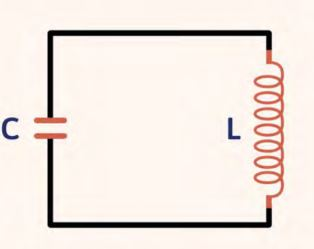
\includegraphics[scale=0.5]{../figs/4-1-1.JPG}
\end{center}
\begin{itemize}
	\item Gồm một tụ điện có điện dung $C$ mắc với một cuộn cảm có độ tự cảm $L$ thành mạch kín.
	\item Nếu điện trở của mạch rất nhỏ, coi như bằng không, thì mạch là một mạch dao động lý tưởng.
\end{itemize}
\subsection{Sự biến thiên điện tích và cường độ dòng điện trong mạch dao động lí tưởng}
Điện tích $q$ của một bản tụ điện và cường độ dòng điện $i$ trong mạch dao động biến thiên điều hòa theo thời gian, $i$ sớm pha $\dfrac{\pi}{2} $ so với $q$.
\begin{equation}
	q=q_0\cos(\omega t +\varphi)\ \text{C}, 
\end{equation}
\begin{equation}
	i=\frac{dq}{dt}=I_0 \cos(\omega +\varphi+ \frac{\pi}{2})\ \text{A},
\end{equation}
trong đó: $I_0=q_0\omega, \omega =\dfrac{1}{\sqrt {LC}}$.
\subsection {Dao động điện từ tự do}
Sự biến thiên điều hòa theo thời gian của điện tích $q$ của một bản tụ điện và cường độ dòng điện $i$ (hoặc cường độ điện trường $\vec{E}$ và cảm ứng từ $\vec{B}$) trong mạch dao động được gọi là dao động điện từ tự do.
\subsection {Chu kì và tần số dao động riêng của mạch dao đông}
Gồm tụ điện có điện dung $C$ mắc với một cuộn cảm có độ tự cảm $L$ thành mạch kín.
\begin{equation}
	T=2\pi \sqrt {LC},
\end{equation}
\begin{equation}
	f=\frac{1}{2\pi\sqrt {LC}},
\end{equation}
trong đó:\\
$L$: Độ tự cảm của cuộn dây ($\text{H}$);\\
$C$: Điện dung của tụ điện ($\text{F}$);\\
$T$: Chu kì dao động ($\text{s}$);\\
$f$: Tần số dao động riêng của mạch dao động ($\text{Hz}$).
\subsection {Năng lượng điện từ}
\begin{itemize}
	\item Tổng năng lượng điện trường trong tụ điện và năng lượng từ trường trong cuộn cảm của mạch gọi là năng lượng điện từ.\\
	\begin{equation}
		W=W_{\text{đ}}+W_{t}=\frac{1}{2}Cu^2+\frac{1}{2}Li^2
	\end{equation}
	\item Nếu không có sự tiêu hao năng lượng thì năng lượng điện từ trong mạch sẽ được bảo toàn.
\end{itemize}
\section{Mục tiêu bài học - Ví dụ minh họa}
\begin{dang}{Xác định chu kỳ, tần số, điện tích của mạch dao động}
	\viduii{2}{
		
		Mạch dao động LC lí tưởng gồm cuộn cảm có độ tự cảm $L = \SI{2}{mH}$ và tụ điện có điện dung $C = \SI{2}{pF}$. Tần số dao động của mạch gần bằng
		\begin{mcq}(4)
			\item $\SI{1}{MHz}$. 
			\item $\SI{2,5}{MHz}$. 
			\item $\SI{1}{kHz}$. 
			\item $\SI{2,5}{kHz}$. 
		\end{mcq}
	}
	{	\begin{center}
			\textbf{Hướng dẫn giải}
		\end{center}
		
		
		Tần số dao động riêng của mạch cho bởi
		
		$$f = \dfrac{1}{2\pi \sqrt{LC}} = \SI{2,5}{MHz}.$$
		
		\textbf{Đáp án: B.}
		
		
		\begin{center}
			\textbf{Câu hỏi tương tự}
		\end{center}
		
		Một mạch dao động gồm một cuộn cảm có độ tự cảm $L = \SI{1}{mH}$ và một tụ điện có điện dung là $C = \SI{0,1}{\mu F}$. Tần số riêng của mạch có giá trị nào?
		
		\textbf{Đáp án:} $f = \text{1,6}\cdot 10^4\ \text{Hz}$.
	}
	\viduii{2}{
		
		Mạch dao động điện từ lí tưởng gồm cuộn dây thuần cảm có độ tự cảm L và tụ điện có điện dung C. Khi tăng điện dung của tụ điện lên 9 lần thì chu kì dao động riêng của mạch
		\begin{mcq}(2)
			\item tăng lên 9 lần. 
			\item tăng lên 3 lần. 
			\item giảm đi 9 lần. 
			\item giảm 3 lần. 
		\end{mcq}
	}
	{	\begin{center}
			\textbf{Hướng dẫn giải}
		\end{center}
		
		Ban đầu, chu kì dao động riêng của mạch cho bởi công thức 
		
		$$T = 2\pi \sqrt{LC}.$$
		
		Lúc sau, chu kì dao động riêng của mạch cho bởi công thức 
		
		$$T' = 2\pi \sqrt{LC'}.$$ 
		
		Lập tỉ lệ hai biểu thức trên ta được
		
		$$\dfrac{T'}{T} = \sqrt{\dfrac{C'}{C}}.$$
		
		Thay $C' = 9C$ vào biểu thức trên ta được $T' = 3T$.
		
		\textbf{Đáp án: B.}
		
		\begin{center}
			\textbf{Câu hỏi tương tự}
		\end{center}
		
		Mạch dao động điện từ điều hoà gồm cuộn cảm $L$ và tụ điện $C$, khi tăng điện dung của tụ điện lên 4 lần thì chu kỳ dao động của mạch?
		
		\textbf{Đáp án:} tăng lên 2 lần.
	}
	
	
	\viduii{2}{
		Một mạch dao động lí tưởng gồm cuộn cảm thuần có độ tự cảm $\xsi{4}{\mu H}$ và một tụ điện có điện dung biến đổi từ $\xsi{10}{pF}$ đến $\xsi{640}{pF}$. Lấy $\pi^2 = 10$. Chu kì dao động riêng của mạch có giá trị
		\begin{mcq}(2)
			\item từ $\xsi{4,2\cdot10^{-8}}{s}$ đến $\xsi{2,4\cdot10^{-7}}{s}$. 
			\item từ $\xsi{2,24\cdot10^{-8}}{s}$ đến $\xsi{3\cdot10^{-7}}{s}$. 
			\item từ $\xsi{2\cdot10^{-8}}{s}$ đến $\xsi{3,6\cdot10^{-7}}{s}$. 
			\item từ $\xsi{4\cdot10^{-8}}{s}$ đến $\xsi{3,2\cdot10^{-7}}{s}$. 
		\end{mcq}
	}
	{	\begin{center}
			\textbf{Hướng dẫn giải}
		\end{center}
		
		Chu kì dao động riêng trong mạch cho bởi: 
		
		$$T = 2\pi \sqrt{LC}.$$
		
		Khi $C = \xsi{10}{pF}$, ta có:
		
		$$T = 2\pi \sqrt{LC} = \xsi{4\cdot10^{-8}}{s}.$$ 
		
		Khi $C = \xsi{640}{pF}$, ta có:
		
		$$T = 2\pi \sqrt{LC} = \xsi{3,2\cdot10^{-7}}{s}.$$ 
		
		Vậy chu kì dao động riêng của mạch biến thiên từ $\xsi{4\cdot10^{-8}}{s}$ đến $\SI{3,2 e-7}{s}$.
		
		\textbf{Đáp án: D.}
		
		\begin{center}
			\textbf{Câu hỏi tương tự}
		\end{center}
		
		Một mạch dao động lí tưởng gồm tụ điện có điện dung $C$ và cuộn cảm thuần có độ tự cảm $L$, đang thực hiện dao động điện từ tự do với tần số $f$. Nếu tăng điện dung của tụ điện lên 16 lần thì tần số dao động của mạch giảm lượng $\SI{24}{MHz}$. Giá trị của $f$ bằng
		\begin{mcq}(4)
			\item $\SI{48}{MHz}$. 
			\item $\SI{32}{MHz}$. 
			\item $\SI{40}{MHz}$. 
			\item $\SI{36}{MHz}$. 
		\end{mcq}
		
		\textbf{Đáp án: B}.
	}
	\viduii{2}{
		Điện tích của một bản tụ trong mạch dao động $LC$ lí tưởng biến đổi điều hòa có biểu thức là $q = 6\cdot10^{-6} \cos \left( 4000t + \dfrac{\pi}{2} \right)\ \text C$. Tại thời điểm $t = \xsi{10^{-4}}{s}$, điện tích trên bản tụ có độ lớn xấp xỉ bằng 
		\begin{mcq}(2)
			\item $\SI{2,30e-6}{C}$. 
			\item $\SI{5,90e-6}{C}$. 
			\item $\SI{1,15e-6}{C}$. 
			\item $\SI{4,60e-6}{C}$. 
		\end{mcq}
	}
	{	\begin{center}
			\textbf{Hướng dẫn giải}
		\end{center}
		
		Ta thay thời điểm $t = \SI{e-4}{s}$ vào biểu thức điện tích, ta được:
		
		$$ q = \num{6e-6} \cos \left( 4000t + \dfrac{\pi}{2} \right) = -\SI{2,30 e-6}{C}.$$
		
		\textbf{Đáp án: A.}
		
		\begin{center}
			\textbf{Câu hỏi tương tự}
		\end{center}
		
		Điện tích của một bản tụ trong mạch dao động $LC$ đang thực hiện dao động điện từ tự do là $q = 4\cdot10^{-7} \cos \left( 4000t \right)\ \text C$. Điện tích cực đại có độ lớn
		\begin{mcq}(2)
			\item $\xsi{2\sqrt{2}\cdot10^{3}}{C}$. 
			\item $\xsi{22\cdot10^{-7}}{C}$. 
			\item $\xsi{4\cdot10^{-7}}{C}$. 
			\item $\xsi{4\cdot10^{3}}{C}$. 
		\end{mcq}
		
		\textbf{Đáp án: C}.
	}
	
	\viduii{2}{
		
		Một mạch dao động lí tưởng gồm tụ điện có điện dung $C = 2 \mu \text F$ và cuộn cảm thuần có độ tự cảm $L$, đang thực hiện dao động điện từ tự do. Biết dòng điện qua mạch có dạng $i = 2 \cos \left( 5000t \right)\ \text{mA}$. Giá trị của $L$ bằng
		\begin{mcq}(4)
			\item $\SI{0,05}{H}$. 
			\item $\SI{0,01}{H}$. 
			\item $\SI{0,02}{H}$. 
			\item $\SI{0,04}{H}$. 
		\end{mcq}
	}
	{	\begin{center}
			\textbf{Hướng dẫn giải}
		\end{center}
		
		Tần số dao động riêng của mạch 
		
		$$\omega = \SI{5000}{rad/s}.$$ 
		
		Lại có $\omega = \dfrac{1}{\sqrt{LC}}$ nên suy ra
		
		$$L = \dfrac{1}{C \omega^2} = \SI{0,02}{H}.$$ 
		
		\textbf{Đáp án: C.}
		
		\begin{center}
			\textbf{Câu hỏi tương tự}
		\end{center}
		
		Điện tích của một bản tụ trong mạch dao động điện từ có phương trình là $q = Q_0 \cos \left( 4\pi \cdot 10^{4}t \right)\ \text C$. Trong đó $t$ tính theo giây. Tần số dao động của mạch là
		\begin{mcq}(2)
			\item $ \SI{1e4}{Hz} $.
			\item $ \SI{20e14}{Hz} $.
			\item $ \SI{2e4}{Hz} $.
			\item $ \SI{2e4}{kHz} $.
		\end{mcq}
		
		\textbf{Đáp án: C}.
	}
	
\end{dang}

\begin{dang}{Xác định năng lượng điện từ của mạch dao động}
	\viduii{2}{
		
		Một mạch dao động $LC$ có điện trở thuần không đáng kể, tụ điện có điện dung $\SI{5}{\mu \text F}$. Dao động điện từ tự do của mạch $LC$ với hiệu điện thế cực đại ở hai đầu tụ điện bằng $\SI{6}{V}$. Khi hiệu điện thế ở hai đầu tụ điện là $\SI{4}{V}$ thì năng lượng điện từ trong mạch bằng
		\begin{mcq}(4)
			\item $\xsi{9\cdot10^{-5}}{J}$. 
			\item $\xsi{5\cdot10^{-5}}{J}$. 
			\item $\xsi{4\cdot10^{-5}}{J}$. 
			\item $\xsi{10^{-5}}{J}$. 
		\end{mcq}
	}
	{	\begin{center}
			\textbf{Hướng dẫn giải}
		\end{center}
		
		Năng lượng điện từ trong mạch ở thời điểm bất kì cũng chính là năng lượng cực đại của điện trường bên trong tụ điện:
		
		$$W = W_C = \dfrac{1}{2}CU^{2} = \xsi{9\cdot10^{-5}}{J}.$$
		
		\textbf{Đáp án: A.}
		
		\begin{center}
			\textbf{Câu hỏi tương tự}
		\end{center}
		
		Một mạch dao động $LC$ có cuộn thuần cảm có độ tự cảm $L = \SI{0,4}{H}$ và tụ điện có điện dung $C= \SI{40}{\mu F}$ Cường độ dòng điện qua mạch có biểu thức: $i = 2\sqrt 2 \cos 100\pi t\ \text A$. Tính năng lượng dao động của mạch?
		
		\textbf{Đáp án:} $W = \SI{1,6}{J}.$
	}
	\viduii{2}{
		
		Cho một mạch dao động điện từ gồm một tụ điện có điện dung $C = \SI{5}{\mu F}$ và một cuộn thuần cảm có độ tự cảm $L = \SI{50}{mH}$. Biết điện áp cực đại trên tụ là  $\SI{6}{V}$. Tìm năng lượng điện trường và năng lượng từ trường trong mạch khi điện áp trên tụ điện là $\SI{4}{V}$ và cường độ dòng điện $i$ khi đó.
		
	}
	{	\begin{center}
			\textbf{Hướng dẫn giải}
		\end{center}
		
		Năng lượng điện trường
		
		$$W_\text{đ} = \dfrac{1}{2} Cu^2 = 4 \cdot 10^{-5}\ \text{J}.$$
		
		Năng lượng điện từ
		
		$$W = \dfrac{1}{2}CU_0^2 = 9 \cdot 10^{-5}\ \text J.$$
		
		Cường độ dòng điện $i$
		
		$$ W_\text t =\dfrac{1}{2} Li^2 \Rightarrow i = \SI{0,045}{A}.$$
		
		\begin{center}
			\textbf{Câu hỏi tương tự}
		\end{center}
		
		Trong một mạch $LC$, $L = \SI{25}{mH}$ và $C = \SI{1,6}{\mu F}$ ở thời điểm $t = 0$, cường độ dòng điện trong mạch bằng $\SI{6,93}{mA}$, điện tích ở trên tụ điện bằng $\SI{0,8}{\mu C}$. Tính năng lượng của mạch dao động.
		
		\textbf{Đáp án:} $W = \text{0,8}\cdot 10^{-6}\ \text J.$
	}
	
\end{dang}
\section{Bài tập tự luyện}
\begin{enumerate}[label=\bfseries Câu \arabic*:]
	%------------------------------------------------------------------------------------------
	\item \mkstar{1} [1] %Cau 1
	
	{Một mạch dao động lí tưởng gồm tụ điện có điện dung $C$ và cuộn cảm thuần có độ tự cảm $L$, đang thực hiện dao động điện từ tự do. Biết dòng điện qua mạch có dạng $i = I_0 \cos \left( \omega t \right)$. Điện tích tụ điện có giá trị cực đại bằng
		\begin{mcq}(4)
			\item $I_0 \sqrt{\omega}$. 
			\item $\dfrac{I_0}{\sqrt{\omega}}$.
			\item $\dfrac{I_0}{\omega}$. 
			\item $\omega I_o$. 
		\end{mcq}
	}
	
	\hideall
	{		\textbf{Đáp án: C.}
		
		Mối quan hệ giữa cường độ dòng điện cực đại trong mạch $I_0$ và điện tích cực đại trên bản tụ $Q_0$ là $I_0 = \omega Q_0$. Vậy nên điện tích cực đại trên bản tụ là 
		$$Q_0 = \dfrac{I_0}{\omega}.$$
		
	}
	
	%--------------------------------------------------------------------------------------------------------------
	%--------------------------------------------------------------------------------------------------------------
	\item \mkstar{1} [2] %Cau 2
	{Trong máy thu thanh vô tuyến, bộ phận dùng để biến đổi trực tiếp dao động điện thành dao động âm có cùng tần số là
		\begin{mcq}(4)
			\item mạch tách sóng. 
			\item mạch chọn sóng. 
			\item micrô. 
			\item loa. 
		\end{mcq}
	}
	
	\hideall
	{		\textbf{Đáp án: D.}
		
		Trong máy thu thanh vô tuyến, bộ phận dùng để biến đổi trực tiếp dao động điện thành dao động âm có cùng tần số là loa.
		
	}
	
	%--------------------------------------------------------------------------------------------------------------
	%--------------------------------------------------------------------------------------------------------------
	\item \mkstar{1} [2] %Cau 3
	
	{Mạch dao động điện từ lí tưởng, cuộn cảm có độ tự cảm L và tụ điện có điện dung C. Chu kì dao động là
		\begin{mcq}(4)
			\item $T = \dfrac{2\pi}{\sqrt{LC}}$. 
			\item $T = \sqrt{LC}$. 
			\item $T = 2\pi \sqrt{LC}$. 
			\item $T = \dfrac{1}{2\pi \sqrt{LC}}$. 
		\end{mcq}
	}
	
	\hideall
	{		\textbf{Đáp án: C.}
		
		Công thức  tính chu kì dao động của vật là $T = 2\pi \sqrt{LC}$.
		
	}
	
	%--------------------------------------------------------------------------------------------------------------
	%--------------------------------------------------------------------------------------------------------------
	\item \mkstar{1} [4] %Cau 4
	
	{Trong mạch dao động điện từ lí tưởng đang hoạt động, điện tích trên một bản tụ điện biến thiên điều hòa
		\begin{mcq}(1)
			\item cùng pha với cường độ dòng điện trong đoạn mạch. 
			\item lệch pha $\text{0,25} \pi$ so với cường độ dòng điện trong đoạn mạch. 
			\item ngược pha với cường độ dòng điện trong đoạn mạch. 
			\item lệch pha $\text{0,5} \pi$ so với cường độ dòng điện trong đoạn mạch. 
		\end{mcq}
	}
	
	\hideall
	{		\textbf{Đáp án: D.}
		
		Trong mạch dao động đang hoạt động, cường độ dòng điện luôn sớm pha $\pi /2$ so với điện tích trên một bản tụ.
		
	}
	
	%--------------------------------------------------------------------------------------------------------------
	%--------------------------------------------------------------------------------------------------------------
	\item \mkstar{1} [12] %Cau 5
	
	{Trong mạch dao động  $LC$ lí tưởng $L$ và $C$ thay đổi được, muốn giảm tần số dao động riêng của mạch thì có thể
		\begin{mcq}(2)
			\item tăng $C$, giữ nguyên $L$. 
			\item giảm $C$ một nửa, tăng $L$ gấp 2 lần. 
			\item giảm $C$ và giảm $L$. 
			\item giảm $C$ và giữ nguyên $L$. 
		\end{mcq}
	}
	
	\hideall
	{		\textbf{Đáp án: A.}
		
		Công thức tính tần số dao động riêng là
		$$
		f = \dfrac{1}{2\pi \sqrt{LC}}.
		$$ \\
		Vậy nên, để giảm tần số dao động riêng $f$, ta tăng $C$ và giữ nguyên $L$.
	}
	
	%--------------------------------------------------------------------------------------------------------------
	%--------------------------------------------------------------------------------------------------------------
	\item \mkstar{1} [7] %Cau 6
	
	{Một mạch dao động LC lí tưởng đang có dao động điện từ tự do với tần số góc $\omega$. Gọi $q_0$ là điện tích cực đại của một bản tụ điện thì cường độ dòng điện cực đại trong mạch là
		\begin{mcq}(4)
			\item $\dfrac{q_0}{\omega^2}$. 
			\item $q_0 \omega^2$. 
			\item $q_0 \omega$. 
			\item $\dfrac{q_0}{\omega}$. 
		\end{mcq}
	}
	
	\hideall
	{		\textbf{Đáp án: C.}
		
		Mối liên hệ giữa điện tích cực đại $q_0$ và cường độ dòng điện cực đại $I_0$ là
		$$
		I_0 = \omega q_0.
		$$
		
	}	
	
	%--------------------------------------------------------------------------------------------------------------
	%--------------------------------------------------------------------------------------------------------------
	\item \mkstar{1} [7] %Cau 7
	
	{Trong mạch dao động điện từ tự do $LC$, so với cường độ dòng điện trong mạch thì điện tích trên một bản tụ luôn
		\begin{mcq}(2)
			\item trễ pha hơn một góc $\pi/2$. 
			\item sớm pha hơn một góc $\pi/2$. 
			\item cùng pha. 
			\item sớm pha hơn một góc $\pi/4$. 
		\end{mcq}
	}
	
	\hideall
	{		\textbf{Đáp án: A.}
		
		Trong mạch dao động điện từ tự do $LC$, so với cường độ dòng điện trong mạch thì điện tích trên một bản tụ luôn trễ pha hơn một góc $\pi/2$.
		
	}
	
	%--------------------------------------------------------------------------------------------------------------
	%--------------------------------------------------------------------------------------------------------------
	\item \mkstar{1} [7]
	
	{Một mạch dao động gồm cuộn cảm thuần có độ tự cảm L và tụ điện có điện dung C. Chu kì dao động riêng của mạch là
		\begin{mcq}(4)
			\item $\dfrac{\sqrt{LC}}{2\pi}$. 
			\item $2\pi \sqrt{LC}$. 
			\item $\dfrac{1}{2\pi \sqrt{LC}}$. 
			\item $\dfrac{2\pi}{\sqrt{LC}}$. 
		\end{mcq}
	}
	
	\hideall
	{		\textbf{Đáp án: B.}
		
		Chu kì dao động riêng của mạch dao động là $2\pi \sqrt{LC}$.
		
	}	
	
	%--------------------------------------------------------------------------------------------------------------
	%--------------------------------------------------------------------------------------------------------------
	\item \mkstar{1} [12]
	
	{Điện tích của một bản tụ trong mạch dao động LC đang thực hiện dao động điện từ tự do là $q = 4\cdot10^{-7} \cos \left( 4000t \right)$ (C). Điện tích cực đại có độ lớn
		\begin{mcq}(4)
			\item $\xsi{2\sqrt{2}\cdot10^{3}}{C}$. 
			\item $\xsi{22\cdot10^{-7}}{C}$. 
			\item $\xsi{4\cdot10^{-7}}{C}$. 
			\item $\xsi{4\cdot10^{3}}{C}$. 
		\end{mcq}
	}
	
	\hideall
	{		\textbf{Đáp án: C.}
		
		Từ biểu thức của cường độ dòng điện $q = 4\cdot10^{-7} \cos \left( 4000t \right)$ (C) ta suy ra điện tích cực đại trên bản tụ điện là $\xsi{4\cdot10^{-7}}{C}$.
		
	}
	
	%--------------------------------------------------------------------------------------------------------------
	%--------------------------------------------------------------------------------------------------------------
	\item \mkstar{2} [3]
	
	{Gọi $I_0$ và $Q_0$ là giá trị cực đại của điện tích trên bản tụ và cường độ dòng điện cực đại trong mạch dao động điện từ LC. Chu kì dao động điện từ tự do trong mạch có biểu thức
		\begin{mcq}(4)
			\item $T = \dfrac{2\pi}{I_0 Q_0}$. 
			\item $T = \dfrac{2\pi Q_0}{I_0}$. 
			\item $T = 2\pi\sqrt{Q_0 I_0}$. 
			\item $T = 2\pi Q_0 I_0$. 
		\end{mcq}
	}
	
	\hideall
	{		\textbf{Đáp án: B.}
		
		Ta có chu kì dao động tự do của mạch cho bởi $T = \dfrac{2\pi}{\omega}$. \\
		Lại có $\omega = \dfrac{I_0}{Q_0}$. \\
		Từ đó:
		$$T = \dfrac{2\pi}{\omega} = \dfrac{2\pi}{\dfrac{I_0}{Q_0}} = \dfrac{2\pi Q_0}{I_0}.$$
		
	}
	
	%--------------------------------------------------------------------------------------------------------------
	%--------------------------------------------------------------------------------------------------------------
	\item \mkstar{2} [12]
	
	{Điện tích của một bản tụ trong mạch dao động LC lí tưởng là $q = 6\cdot10^{-6} \cos \left( 4000t + \dfrac{\pi}{2} \right)$ (C). Tại thời điểm $t = \xsi{10^{-4}}{s}$, điện tích trên bản tụ có độ lớn xấp xỉ bằng 
		\begin{mcq}(4)
			\item $\SI{2,30e-6}{C}$. 
			\item $\SI{5,90e-6}{C}$. 
			\item $\SI{1,15e-6}{C}$. 
			\item $\SI{4,60e-6}{C}$. 
		\end{mcq}
	}
	
	\hideall
	{		\textbf{Đáp án: A.}
		
		Ta thay thời điểm $t = \SI{e-4}{s}$ vào biểu thức điện tích, ta được:
		$$
		q = \num{6e-6} \cos \left( 4000t + \dfrac{\pi}{2} \right) = \num{6e-6}\cos \left( 4000\cdot10^{-4} + \dfrac{\pi}{2} \right) = -\SI{2,30 e-6}{C}
		$$
		
	}
	
	%--------------------------------------------------------------------------------------------------------------
	%--------------------------------------------------------------------------------------------------------------
	\item \mkstar{2} [9]
	
	{Một mạch dao động LC có điện trở thuần không đáng kể, tụ điện có điện dung $\SI{5}{\mu F}$. Dao động điện từ tự do của mạch LC với hiệu điện thế cực đại ở hai đầu tụ điện bằng $\SI{6}{V}$. Khi hiệu điện thế ở hai đầu tụ điện là $\SI{4}{V}$ thì năng lượng điện từ trong mạch bằng
		\begin{mcq}(4)
			\item $\xsi{9\cdot10^{-5}}{J}$. 
			\item $\xsi{5\cdot10^{-5}}{J}$. 
			\item $\xsi{4\cdot10^{-5}}{J}$. 
			\item $\xsi{10^{-5}}{J}$. 
		\end{mcq}
	}
	
	\hideall
	{		\textbf{Đáp án: A.}
		
		Năng lượng điện từ trong mạch ở thời điểm bất kì cũng chính là năng lượng cực đại của điện trường bên trong tụ điện:
		$$
		W = W_C = \dfrac{1}{2}CU^{2} = \dfrac{1}{2} \cdot 5\cdot10^{-6} \cdot 6^{2} = \xsi{9\cdot10^{-5}}{J}.
		$$
	}
	
	%------------------------------------------------------------------------------------------
	\item \mkstar{2} [7]
	
	{Mạch dao động LC lí tưởng gồm cuộn cảm có độ tự cảm $L = \SI{2}{mH}$ và tụ điện có điện dung $C = \SI{2}{pF}$. Tần số dao động của mạch gần bằng
		\begin{mcq}(4)
			\item $\SI{1}{MHz}$. 
			\item $\SI{2,5}{MHz}$. 
			\item $\SI{1}{kHz}$. 
			\item $\SI{2,5}{kHz}$. 
		\end{mcq}
	}
	
	\hideall
	{		\textbf{Đáp án: B.}
		
		Tần số dao động riêng của mạch cho bởi
		$$
		f = \dfrac{1}{2\pi \sqrt{LC}} = \dfrac{1}{2\pi \sqrt{2\cdot 10^{-3} \cdot 2\cdot 10^{-12}}} = \SI{2,5}{MHz}.
		$$
		
	}
	
	
	%--------------------------------------------------------------------------------------------------------------
	%--------------------------------------------------------------------------------------------------------------
	\item \mkstar{2} [4]
	
	{Mạch dao động điện từ lí tưởng gồm cuộn dây thuần cảm có độ tự cảm L và tụ điện có điện dung C. Khi tăng điện dung của tụ điện lên 9 lần thì chu kì dao động riêng của mạch
		\begin{mcq}(4)
			\item tăng lên 9 lần. 
			\item tăng lên 3 lần. 
			\item giảm đi 9 lần. 
			\item giảm 3 lần. 
		\end{mcq}
	}
	
	\hideall
	{		\textbf{Đáp án: B.}
		
		Ban đầu, chu kì dao động riêng của mạch cho bởi công thức $T = 2\pi \sqrt{LC}$. \\
		Lúc sau, chu kì dao động riêng của mạch cho bởi công thức $T' = 2\pi \sqrt{LC'}$. \\
		Lập tỉ lệ hai biểu thức trên ta được $\dfrac{T'}{T} = \sqrt{\dfrac{C'}{C}}$. \\
		Thay $C' = 9C$ vào biểu thức trên ta được $T' = 3T$.
		
	}
	
	%--------------------------------------------------------------------------------------------------------------
	%--------------------------------------------------------------------------------------------------------------
	\item \mkstar{2} [10]
	
	{Coi dao động điện từ của một mạch dao động LC là dao động tự do. Biết độ tự cảm của cuộn dây là $\xsi{2\cdot10^{-2}}{H}$, điện dung tụ điện là $\xsi{2\cdot10^{-10}}{F}$. Chu kì dao động điện từ tự do trong mạch này là
		\begin{mcq}(4)
			\item $\xsi{4\pi . 10^{-6}}{s}$. 
			\item $\xsi{2\pi . 10^{-6}}{s}$. 
			\item $\xsi{4\pi}{s}$. 
			\item $\xsi{2\pi}{s}$. 
		\end{mcq}
	}
	
	\hideall
	{		\textbf{Đáp án: A.}
		
		Chu kì dao động riêng của mạch cho bởi:
		$$T = 2\pi \sqrt{LC} = 2\pi \sqrt{2\cdot10^{-2} \cdot 2\cdot10^{-10}} = \xsi{4\pi . 10^{-6}}{s}$$.
		
	}
	
	%--------------------------------------------------------------------------------------------------------------
	%--------------------------------------------------------------------------------------------------------------
	\item \mkstar{2} [10]
	
	{Mạch dao động điện từ LC lí tưởng gồm cuộn thuần cảm có độ tự cảm $\xsi{1}{mH}$ và tụ điện có điện dung $\xsi{0,1}{\mu F}$. Dao động điện từ riêng của mạch có tần số góc là
		\begin{mcq}(4)
			\item $\xsi{2\cdot10^{5}}{rad/s}$. 
			\item $\xsi{10^{5}}{rad/s}$. 
			\item $\xsi{3\cdot10^{5}}{rad/s}$. 
			\item $\xsi{4\cdot10^{5}}{rad/s}$. 
		\end{mcq}
	}
	
	\hideall
	{		\textbf{Đáp án: B.}
		
		Tần số góc dao động riêng của mạch cho bởi:
		$$\omega = \dfrac{1}{\sqrt{LC}} = \dfrac{1}{\sqrt{1\cdot10^{-3}\cdot \text{0,1}\cdot10^{-6}}} = \xsi{10^{5}}{rad/s}.$$
		
	}
	
	%--------------------------------------------------------------------------------------------------------------
	%--------------------------------------------------------------------------------------------------------------
	\item \mkstar{2} [1] %Cau17
	
	{Một mạch dao động lí tưởng gồm tụ điện có điện dung $C = 2 \mu F$ và cuộn cảm thuần có độ tự cảm $L$, đang thực hiện dao động điện từ tự do. Biết dòng điện qua mạch có dạng $i = 2 \cos \left( 5000t \right)(mA,s)$. Giá trị của L bằng
		\begin{mcq}(4)
			\item $\SI{0,05}{H}$. 
			\item $\SI{0,01}{H}$. 
			\item $\SI{0,02}{H}$. 
			\item $\SI{0,04}{H}$. 
		\end{mcq}
	}
	
	\hideall
	{		\textbf{Đáp án: C.}
		
		Từ phương trình dòng điện qua mạch $i = 2 \cos \left( 5000t \right)$ (mA,s) ta rút ra tần số dao động riêng của mạch $\omega = \SI{5000}{rad/s}$. \\
		Lại có $\omega = \dfrac{1}{\sqrt{LC}}$ nên suy ra 
		$$L = \dfrac{1}{C \omega^2} = \dfrac{1}{2\cdot10^{-6} \cdot 5000^2} = \SI{0,02}{H}.$$ 
		
	}
	
	%--------------------------------------------------------------------------------------------------------------
	%--------------------------------------------------------------------------------------------------------------
	\item \mkstar{2} [2] %Cau18
	
	{Điện tích của một bản tụ trong mạch dao động điện từ có phương trình là $q = Q_0 \cos \left( 4\pi \cdot 10^{4}t \right)$. Trong đó $t$ tính theo giây. Tần số dao động của mạch là
		\begin{mcq}(4)
			\item $ \SI{1e4}{Hz} $.
			\item $ \SI{20e14}{Hz} $.
			\item $ \SI{2e4}{Hz} $.
			\item $ \SI{2e4}{kHz} $.
		\end{mcq}
	}
	
	\hideall
	{		\textbf{Đáp án: C.}
		
		Từ phương trình $q = Q_0 \cos \left( 4\pi \cdot 10^{4}t \right)$ ta rút ra tần số góc của mạch là $\omega = \xsi{4 \pi e4}{rad/s}.$ \\
		Tần số dao động của mạch cho bởi
		$$f = \dfrac{\omega}{2\pi} = \dfrac{4\pi \cdot 10^{4}}{2\pi} = \SI{2 e4}{Hz}.$$
		
	}
	
	%--------------------------------------------------------------------------------------------------------------
	%--------------------------------------------------------------------------------------------------------------
	\item \mkstar{3} [10] %Cau19
	
	{Một mạch dao động lí tưởng gồm cuộn cảm thuần có độ tự cảm $\xsi{4}{\mu H}$ và một tụ điện có điện dung biến đổi từ $\xsi{10}{pF}$ đến $\xsi{640}{pF}$. Lấy $\pi^2 = 10$. Chu kì dao động riêng của mạch có giá trị
		\begin{mcq}(2)
			\item từ $\xsi{4,2\cdot10^{-8}}{s}$ đến $\xsi{2,4\cdot10^{-7}}{s}$. 
			\item từ $\xsi{2,24\cdot10^{-8}}{s}$ đến $\xsi{3\cdot10^{-7}}{s}$. 
			\item từ $\xsi{2\cdot10^{-8}}{s}$ đến $\xsi{3,6\cdot10^{-7}}{s}$. 
			\item từ $\xsi{4\cdot10^{-8}}{s}$ đến $\xsi{3,2\cdot10^{-7}}{s}$. 
		\end{mcq}
	}
	
	\hideall
	{		\textbf{Đáp án: D.}
		
		Chu kì dao động riêng trong mạch cho bởi: $T = 2\pi \sqrt{LC}$. \\
		Khi $C = \xsi{10}{pF}$, ta có:
		$$
		T = 2\pi \sqrt{LC} = 2\pi \sqrt{4\cdot10^{-6} \cdot 10\cdot10^{-12}} = \xsi{4\cdot10^{-8}}{s}.
		$$ \\
		Khi $C = \xsi{640}{pF}$, ta có;
		$$
		T = 2\pi \sqrt{LC} = 2\pi \sqrt{4\cdot10^{-6} \cdot 640\cdot10^{-12}} = \xsi{3,2\cdot10^{-7}}{s}.
		$$ \\
		Vậy chu kì dao động riêng của mạch biến thiên từ $\xsi{4\cdot10^{-8}}{s}$ đến $\SI{3,2 e-7}{s}$.
	}
	
	%--------------------------------------------------------------------------------------------------------------
	%--------------------------------------------------------------------------------------------------------------
	\item \mkstar{3} [1] %Cau20
	
	{Một mạch dao động lí tưởng gồm tụ điện có điện dung $C$ và cuộn cảm thuần có độ tự cảm $L$, đang thực hiện dao động điện từ tự do với tần số $f$. Nếu tăng điện dung của tụ điện lên 16 lần thì tần số dao động của mạch giảm lượng $\SI{24}{MHz}$. Giá trị của $f$ bằng
		\begin{mcq}(4)
			\item $\SI{48}{MHz}$. 
			\item $\SI{32}{MHz}$. 
			\item $\SI{40}{MHz}$. 
			\item $\SI{36}{MHz}$. 
		\end{mcq}
	}
	
	\hideall
	{		\textbf{Đáp án: B.}
		
		Ban đầu, tần số dao động riêng của mạch cho bởi 
		$$f = \dfrac{1}{2\pi \sqrt{LC}}.$$
		Lúc sau, khi tăng điện dung của tụ điện lên 16 lần, tần số dao động riêng của mạch là
		$$f' = \dfrac{1}{2\pi \sqrt{LC'}}.$$
		Lập tỉ lệ giữa hai biểu thức trên, ta được:
		$$\dfrac{f'}{f} = \dfrac{C}{C'}.$$
		Thay $\xsi{f' = f - 24}{MHz}$ và $C' = 16C$, ta được:
		$$\dfrac{f - 24}{f} = \dfrac{C}{16C}.$$
		Sử dụng chức năng Solve trên máy tính cầm tay, ta được:
		$$f = \SI{32}{MHz}.$$
		
	}
		\item \mkstar{1}
	
	{Phát biểu nào sau đây là sai khi nói về năng lượng của mạch dao động điện từ $LC$ có điện trở thuần không đáng kể?
		
		\begin{mcq}
			\item Năng lượng điện từ của mạch dao động biến đổi tuần hoàn theo thời gian.
			\item Năng lượng điện trường và năng lượng từ trường cũng biến thiên tuần hoàn theo một tần số chung.
			\item Năng lượng điện từ của mạch dao động bằng năng lượng điện trường cực đại ở tụ điện.
			\item Năng lượng điện từ của mạch dao động bằng năng lượng từ trường cực đại ở cuộn cảm.
			
		\end{mcq}
	}
	
	\hideall
	{		\textbf{Đáp án: A.}
		
	Khi điện trở thuần không đáng kể khi đó năng lượng điện từ được bảo toàn nên A sai.
		
	}
		\item \mkstar{1}
	
	{
		Phát biểu nào sau đây là sai khi nói về mạch dao động điện từ $LC$ có điện trở thuần không đáng kể?
		
		\begin{mcq}
			\item Năng lượng của mạch dao động gồm năng lượng điện trường tập trung ở tụ điện và năng lượng từ trường tập trung ở cuộn cảm.
			
			\item Năng lượng điện trường và năng lượng từ trường cùng biến thiên tuần hoàn theo một tần số chung là tần số của dao động điện từ.
			
			\item Tại mọi thời điểm, tổng năng lượng điện trường và năng lượng từ trường là không đổi.
			\item  Dao động điện từ trong mạch là một dao động tự do.
			
		\end{mcq}
	}
	
	\hideall
	{		\textbf{Đáp án: B.}
		
		Năng lượng điện trường và năng lượng từ trường cùng biến thiên tuần hoàn theo một tần số chung và gấp đôi tần số của dao động điện từ do đó B sai. 
		
	}
		\item \mkstar{1}
	
	{
		Biểu thức nào sau đây không phải là biểu thức tính năng lượng điện từ trong mạch dao động?
		\begin{mcq}(4)
			\item $W = \dfrac{Q_0^2}{2L}.$
			\item $W = \dfrac{1}{2}CU^2_0.$
			\item $W = \dfrac{1}{2}LI^2_0.$
			\item $W = \dfrac{Q_0^2}{2C}.$
		\end{mcq}
	}
	
	\hideall
	{		\textbf{Đáp án: A.}
		
		
		
	}
		\item \mkstar{1}
	
	{Nhận xét nào sau đây liên quan đến năng lượng điện từ của mạch dao động là đúng? Điện tích trong mạch dao động lí tưởng biến đổi với chu kỳ $T$ thì
		
		
		\begin{mcq}
			\item Năng lượng điện trường biển đối với chu kỳ $2T$.
			\item Năng lượng từ trường biến đổi với chu kỳ $2T$.
			
			\item Năng lượng điện trường biến đổi với chu kỳ $T/2$.
			
			\item Năng lượng điện từ biến đổi với chu kỳ $T/2$.
			
		\end{mcq}
	}
	
	\hideall
	{		\textbf{Đáp án: C.}
		
		
		
	}
		\item \mkstar{2}
	
	{
		Mạch dao động lí tưởng $LC$, cường độ dòng điện cực đại qua cuộn dây là $\SI{36}{mA}$. Khi năng lượng điện trường bằng 3 lần năng lượng từ trường thì cường độ dòng điện qua cuộn dây là
		
		\begin{mcq}(4)
			\item $\SI{18}{mA}$.
			\item $\SI{9}{mA}$.
			\item $\SI{12}{mA}$.
			\item $\SI{36}{mA}$.
		\end{mcq}
	}
	
	\hideall
	{		\textbf{Đáp án: A.}
		
		Khi $W_\text{đ} = 3W_\text{t} \Rightarrow W = 4W_\text{t} \Rightarrow i = \dfrac{I_0}{2} = \SI{18}{mA}.$
		
	}
		\item \mkstar{2}
	
	{
		Một mạch dao động $LC$ có điện trở thuần không đáng kể, tụ điện có điện dung $\SI{5}{\mu F}$. Dao động điện từ tự do của mạch $LC$ với hiệu điện thế cực đại ở hai đầu tụ điện bằng $\SI{6}{V}$. Khi hiệu điện thế ở hai đầu tụ điện là $\SI{4}{V}$ thì năng lượng từ trường trong mạch bằng
		
		\begin{mcq}(4)
			\item $4\cdot 10^{-5}\ \text J$.
			\item $5\cdot 10^{-5}\ \text J$.
			\item $9\cdot 10^{-5}\ \text J$.
			\item $\cdot 10^{-5}\ \text J$.
		\end{mcq}
	}
	
	\hideall
	{		\textbf{Đáp án: B.}
		
		Ta có:
		
		$$W_\text t = W - W_\text{đ} = \dfrac{1}{2}C(U_0^2 - u^2) = \xsi{5\cdot 10^{-5}}{J}.$$
		
	}
		\item \mkstar{2}
	
	{Mạch dao động lí tưởng $LC$ gồm tụ điện có điện dung $C = \SI{25}{nF}$ và cuộn dây có độ tụ cảm $L$. Dòng điện trong mạch biến thiên theo phương trình $i = \text{0,02} \cos 8000 t\ \text A$. Năng lượng điện trường vào thời điểm $t = \dfrac{\pi}{48000}\ \text s$ là
		
		\begin{mcq}(4)
			\item $W_C = \SI{38,5}{\mu J}$.
			\item $W_C = \SI{39,5}{\mu J}.$ 
			\item $W_C = \SI{93,75}{\mu J}.$
			\item $W_C = \SI{36,5}{\mu J}.$
		\end{mcq}
	}
	
	\hideall
	{		\textbf{Đáp án: C.}
		
		Vào thời điểm $t = \dfrac{\pi}{48000}\ \text s$ thì $i = \SI{0,01}{A}.$
		
		Do đó năng lượng điện trường
		
		$$W_\text{đ} = \dfrac{1}{2} L(I_0^2 -i^2) = \dfrac{1}{2} \cdot \dfrac{1}{\omega^2 C} (I_0^2 - i^2) = \SI{93,75}{\mu J}.$$
		
		
	}
		\item \mkstar{2}
	
	{
		Cường độ dòng điện tức thời trong một mạch dao động $LC$ lí tưởng là $i =\text{0,08} \cos 2000 t\ \text A$ với $t$ tính bằng giây. Cuộn dây có độ tự cảm là $L = \SI{50}{mH}$. Tại thời điểm cường độ dòng điện tức thời trong mạch bằng giá trị cường độ dòng điện hiệu dụng thì điện áp giữa hai bản tụ điện có độ lớn bằng:
		
		\begin{mcq}(4)
			\item $4\sqrt 2\ \text V$.
			\item $\SI{2}{V}.$
			\item $2\sqrt 2\ \text V.$
			\item $\SI{4}{V}.$
		\end{mcq}
	}
	
	\hideall
	{		\textbf{Đáp án: A.}
		
		Ta có: 
		
		$$\dfrac{1}{2}LI^2_0 = \dfrac{1}{2} CU^2_0 \Rightarrow U_0 = \sqrt{\dfrac{L}{C}I_0} = \sqrt{L^2\omega^2}I_0 = \SI{8}{V}  \Rightarrow u = 4\sqrt 2\ \text{V}.$$
		
	}
		\item \mkstar{2}
	
	{
		Một mạch dao động điện từ $LC$ lý tưởng đang dao động với điện tích cực đại trên một bản cực của tụ điện là $Q_0$. Cứ sau những khoảng thời gian bằng nhau và bằng $10^{-6}\ \text{s}$ thì năng lượng từ trường lại bằng $\dfrac{Q_0^2}{4C}$. Tần số của mạch dao động là
		
		\begin{mcq}(4)
			\item $\text{2,5}\cdot 10^7\ \text{Hz}$.
			\item $10^6\ \text{Hz}.$
			\item $\text{2,5}\cdot 10^5\ \text{Hz}$.
			\item $10^5\ \text{Hz}.$
		\end{mcq}
	}
	
	\hideall
	{		\textbf{Đáp án: C.}
		
		
		
	}
		\item \mkstar{2}
	
	{
		Trong mạch $LC$ điện tích của tụ điện biến thiên điều hoà với giá trị cực đại bằng $Q_0$. Điện tích của tụ điện khi năng lượng từ trường gấp 3 lần năng lượng điện trường là
		
		\begin{mcq}(4)
			\item $q = \pm \dfrac{Q_0}{3}$.
			\item $q = \pm \dfrac{Q_0}{4}.$
			\item $q = \pm \dfrac{Q_0\sqrt 2}{2}.$
			\item $q = \pm \dfrac{Q_0}{2}.$
		\end{mcq}
	}
	
	\hideall
	{		\textbf{Đáp án: D.}
		
		
		
	}
		\item \mkstar{3}
	
	{
		Cho mạch dao động lí tưởng $LC$. Khoảng thời gian ngắn nhất từ thời điểm năng lượng điện trường cực đại đến thời điểm năng lượng từ trường bằng năng lượng điện trường là
		
		\begin{mcq}(4)
			\item $\Delta t = \dfrac{\pi \sqrt{LC}}{6}.$
			\item $\Delta t = \dfrac{\pi \sqrt{LC}}{8}.$
			\item $\Delta t = \dfrac{\pi \sqrt{LC}}{4}.$
			\item $\Delta t = \dfrac{\pi \sqrt{LC}}{2}.$
		\end{mcq}
	}
	
	\hideall
	{		\textbf{Đáp án: C.}
		
		
		
	}
	\item \mkstar{3}
	
	{
		Một mạch dao động gồm một cuộn dây có độ tự cảm $L = \text{1,2} \cdot 10^{-4}\ \text H$ và một tụ điện có điện dung $C = \SI{3}{nF}$. Do các dây nối và cuộn dây có điện trở tổng cộng $r = \SI{2}{\Omega}$ nên có sự tỏa nhiệt trên mạch. Để duy trì dao động trong mạch không bị tắt dần với điện áp cực đại của tụ $U_0 =\SI{6}{V}$ thì trong một tuần lễ phải cung cấp cho mạch một năng lượng là
		
		
		\begin{mcq}(4)
			\item $\SI{76,67}{J}.$
			\item $\SI{544,32}{J}.$
			\item $\SI{155,25}{J}.$
			\item $\SI{554,42}{J}.$
		\end{mcq}
	}
	
	\hideall
	{		\textbf{Đáp án: B.}
		
		
		
	}
\end{enumerate}

				\let\lesson\undefined
\newcommand{\lesson}{\phantomlesson{Bài 20: Mạch dao động}}
\chapter[ Bài toán tương tự dao động cơ]{ Bài toán tương tự dao động cơ}
\section{Lý thuyết}
- Điện tích $q$ của một bản tụ điện và cường độ dòng điện $i$ trong mạch dao động biến thiên điều hòa theo thời gian, $i$ sớm pha $\dfrac{\pi}{2} $ so với $q$.
\begin{equation}
	q=q_0\cos(\omega t +\varphi)\ \text{C}, 
\end{equation}
\begin{equation}
	i=\frac{dq}{dt}=I_0 \cos(\omega +\varphi+ \frac{\pi}{2})\ \text{A},
\end{equation}
trong đó: $I_0=q_0\omega, \omega =\dfrac{1}{\sqrt {LC}}$.

- Biểu thức hiệu điện thế hai đầu tụ điện

$$ u = \dfrac{q}{C} = U_0 \cos (\omega t + \varphi_u)\ \text{V}.$$

với $U_0 =\dfrac{Q_0}{C}.$

- Công thức độc lập:

$$ \left(\dfrac{q}{Q_0}\right)^2 +  \left(\dfrac{i}{I_0}\right)^2 =1; \left(\dfrac{u}{U_0}\right)^2 +  \left(\dfrac{i}{I_0}\right)^2 =1.$$


\section{Mục tiêu bài học - Ví dụ minh họa}
\begin{dang}{Xác định tần số, chu kỳ của\\ mạch dao động.}
	\viduii{2}{
		Cường độ dòng điện tức thời trong mạch dao động $LC$ có dạng $i = \text{0,5} \cos \left( 3000t \right)$. Tần số dao động riêng của mạch là  
		\begin{mcq}(2)
			\item $\SI{3000}{rad/s}$. 
			\item $\SI{477,46}{Hz}$. 
			\item $\xsi{6000\pi}{Hz}$. 
			\item $\SI{3000}{Hz}$. 
		\end{mcq}
	}
	{	\begin{center}
			\textbf{Hướng dẫn giải}
		\end{center}
		
		Tần số dao động riêng trong mạch cho bởi biểu thức:
		
		$$f=\dfrac{\omega}{2 \pi}= \SI{477,76}{Hz}.$$
		
		\textbf{Đáp án: B.}
		
		\begin{center}
			\textbf{Câu hỏi tương tự}
		\end{center}
		
		Một mạch dao động $LC$ lí tưởng có $L = \SI{20}{mH}$ và $C = \SI{200}{pF}$. Chu kì riêng của dao động điện từ trong mạch xấp xỉ bằng
		\begin{mcq}(2)
			\item $\xsi{1,3\cdot10^{-5}}{s}$. 
			\item $\xsi{1,9\cdot10^{-4}}{s}$. 
			\item $\xsi{12,5\cdot10^{-3}}{s}$. 
			\item $\xsi{3,9\cdot10^{-4}}{s}$. 
		\end{mcq}
		
		\textbf{Đáp án: A.} 
	}
	\viduii{3}{
		
		Một mạch dao động điện từ lí tưởng đang có dao động điện từ tự do. Biết điện tích cực đại trên một bản tụ điện là $\xsi{4\sqrt{2}}{\mu C}$ và cường độ dòng điện cực đại trong mạch là $\xsi{0,5\sqrt{2}}{A}$. Thời gian ngắn nhất để điện tích trên một bản tụ giảm từ giá trị cực đại đến nửa giá trị cực đại là
		\begin{mcq}(4)
			\item $\xsi{\dfrac{4\pi}{3}}{\mu s}$. 
			\item $\xsi{\dfrac{16\pi}{3}}{\mu s}$. 
			\item $\xsi{\dfrac{2\pi}{3}}{\mu s}$. 
			\item $\xsi{\dfrac{8\pi}{3}}{\mu s}$. 
		\end{mcq}
	}
	{	\begin{center}
			\textbf{Hướng dẫn giải}
		\end{center}
		
		Tần số riêng của mạch dao động là 
		
		$$\omega = \dfrac{I_0}{q_0} = \SI{125 e3}{rad/s}.$$ 
		
		Từ đường tròn pha, ta thấy để điện tích trên một bản tụ giảm từ giá trị cực đại đến nửa giá trị cực đại thì vector quay quay được một góc nhỏ nhất là $\Delta \varphi = \pi /3.$ 
		
		Vậy thời gian ngắn nhất để điện tích trên một bản tụ giảm từ giá trị cực đại đến nửa giá trị cực đại là
		
		$$\Delta t = \dfrac{\Delta \varphi}{\omega}  = \xsi{\dfrac{8\pi}{3}}{\mu s}.$$
		
		\textbf{Đáp án: D.}
		\begin{center}
			\textbf{Câu hỏi tương tự}
		\end{center}
		
		Trong mạch dao động $LC$ lí tưởng đang có dao động điện từ tự do. Thời gian ngắn nhất để năng lượng điện trường giảm từ giá trị cực đại xuống còn một nửa giá trị cực đại là $\xsi{1,5\cdot10^{-4}}{s}$. Thời gian ngắn nhất để điện tích trên tụ giảm từ giá trị cực đại xuống còn một nửa giá trị đó là
		\begin{mcq}(2)
			\item $\xsi{2\cdot10^{-4}}{s}$. 
			\item $\xsi{6\cdot10^{-4}}{s}$. 
			\item $\xsi{12\cdot10^{-4}}{s}$. 
			\item $\xsi{3\cdot10^{-4}}{s}$. 
		\end{mcq}
		
		\textbf{Đáp án: A.} 
	}
	\viduii{2}{
		
		Một mạch dao động $LC$ lí tưởng với $L = \SI{2,4}{mH}$ và $C = \SI{1,5}{mF}$. Gọi $I_0$ là cường độ dòng điện cực đại trong mạch. Khoảng thời gian ngắn nhất giữa hai lần liên tiếp mà $i =\dfrac{I_0}{3}$ là
		\begin{mcq}(4)
			\item $\SI{4,76}{ms}$. 
			\item $\SI{4,67}{ms}$. 
			\item $\SI{0,29}{ms}$. 
			\item $\SI{4,54}{ms}$. 
		\end{mcq}
	}
	{	\begin{center}
			\textbf{Hướng dẫn giải}
		\end{center}
		
		Từ đường tròn pha, ta xác định được khoảng thời gian ngắn nhất giữa hai lần liên tiếp $i =\dfrac{I_0}{3}$ là
		
		$$\Delta t=\dfrac{2}{\omega} \arccos \left(\dfrac{i}{I_{0}}\right)=\dfrac{2}{\omega} \arccos \dfrac{1}{3}.$$
		
		Lại có,
		
		$$\omega=\dfrac{1}{\sqrt{L C}} \approx \SI{527}{rad/s}.$$
		
		Khi đó,
		
		$$\Delta t=\dfrac{2}{527} \arccos \dfrac{1}{3}= \xsi{4,67\cdot10^{-3}}{s}.$$
		
		\textbf{Đáp án: B.}
		
		
		\begin{center}
			\textbf{Câu hỏi tương tự}
		\end{center}
		
		Một mạch dao động điện từ lí tưởng đang có dao động điện từ tự do. Tại thời điểm $t = 0$, tụ điện bắt đầu phóng điện. Sau khoảng thời gian ngắn nhất $\Delta t = 10^{-6}\ \text{s}$ thì điện tích trên một bản tụ điện bằng một nửa giá trị cực đại. Tính chu kì dao động riêng của mạch.
		
		\textbf{Đáp án:} $T = 6 \cdot 10^{-6}\ \text s.$
	}
	
	\viduii{2}{
		
		Một mạch dao động lí tưởng gồm cuộn cảm thuần có độ tự cảm $\SI{4}{\mu H}$ và một tụ điện có điện dung biến đổi từ $\SI{10}{pF}$ đến $\SI{360}{pF}$. Lấy $\pi^2 = 10$. Chu kì dao động riêng của mạch có giá trị
		\begin{mcq}(2)
			\item $\xsi{4\cdot10^{-8}}{s}$ đến $\xsi{3,2\cdot10^{-7}}{s}$. 
			\item $\xsi{2\cdot10^{-8}}{s}$ đến $\xsi{3,6\cdot10^{-7}}{s}$. 
			\item $\xsi{4\cdot10^{-8}}{s}$ đến $\xsi{2,4\cdot10^{-7}}{s}$. 
			\item $\xsi{2\cdot10^{-8}}{s}$ đến $\xsi{3\cdot10^{-7}}{s}$. 
		\end{mcq}
	}
	{	\begin{center}
			\textbf{Hướng dẫn giải}
		\end{center}
		
		Chu kì dao động riêng của mạch:
		
		$$T=2 \pi \sqrt{L C}.$$
		
		Khi $C=\SI{10}{pF}$, ta có:
		
		$$T=2 \pi \sqrt{4\cdot10^{-6} \cdot 10\cdot10^{-12}}= \xsi{4\cdot10^{-8}}{s}.$$
		
		Khi $C=\SI{360}{pF}$, ta có:
		
		$$T=2 \pi \sqrt{4\cdot10^{-6} \cdot 360\cdot10^{-12}}= \SI{2,4 e-7}{s}.$$
		
		Vậy chu kì dao động riêng của mạch biến thiên từ $\SI{4 e-8}{s}$ đến $\SI{2,4 e-7}{s}$.
		
		\textbf{Đáp án: C.}
		
		
		\begin{center}
			\textbf{Câu hỏi tương tự}
		\end{center}
		
		Một mạch dao động ở máy vào của một máy thu thanh gồm cuộn thuần cảm có độ tự cảm $\SI{3}{\mu H}$ và tụ điện có điện dung biến thiên trong khoảng $\SI{10}{pF}$ và $\SI{500}{pF}$. Biết rằng, muốn thu tần số riêng của mạch dao động phải bằng tần số của mạch cần thu (để có cộng hưởng). Trong không khí, tốc độ truyền sóng điện từ là $\xsi{3\cdot10^{8}}{m/s}$, máy thu này có thể thu được sóng điện từ trong khoảng
		\begin{mcq}(2)
			\item từ $\SI{100}{m}$ đến $\SI{730}{m}$. 
			\item từ $\SI{10,32}{m}$ đến $\SI{73}{m}$. 
			\item từ $\SI{1,24}{m}$ đến $\SI{73}{m}$. 
			\item từ $\SI{10}{m}$ đến $\SI{73}{m}$. 
		\end{mcq}
		
		\textbf{Đáp án: B.}
		
	}
	
\end{dang}

\begin{dang}{Xác định cường độ dòng điện, hiệu điện thế, điện tích trong mạch dao động.}
	\viduii{3}{
		Một mạch dao động $LC$ có $C = \SI{2}{nF}$ đang thực hiện dao động điện từ tự do. Tại thời điểm $t_1$, cường độ dòng điện trong mạch có độ lớn $\SI{8}{mA}$, tại thời điểm $t_2 = t_1 +\dfrac{T}{4}$, hiệu điện thế giữa hai bản tụ có độ lớn $\SI{6}{V}$. Giá trị của $L$ là 
		\begin{mcq}(4)
			\item $\SI{2,250}{H}$. 
			\item $\SI{1,125}{H}$. 
			\item $\SI{2,250}{mH}$. 
			\item $\SI{1,125}{mH}$. 
		\end{mcq}
	}
	{	\begin{center}
			\textbf{Hướng dẫn giải}
		\end{center}
		
		Ta có thời điểm $t_2$ trễ hơn $\dfrac{T}{4}$ so với thời điểm $t_1$ nên đây là hai thời điểm vuông pha. 
		
		Suy ra $i_2$ vuông pha với $i_1$. 
		
		Mà $u_2$ thì vuông pha với $i_2$. 
		
		Nên $i_1$ và $u_2$ hoặc là cùng pha, hoặc là ngược pha với nhau. 
		
		Nếu chỉ xét độ lớn, ta có:
		
		$$\dfrac{|i_1|}{I_0} = \dfrac{|u_2|}{U_0}.$$ 
		
		Lại có $U_0 = \dfrac{Q_0}{C} = \dfrac{I_0}{\omega C}$. Thay vào biểu thức trên, ta được:
		
		$$\dfrac{|i_1|}{I_0} = \dfrac{|u_2|}{\dfrac{I_0}{\omega C}}.$$
		
		Suy ra 
		
		$$|i_1| = |u_2|\omega C \Rightarrow |i_1| = |u_2|\dfrac{1}{\sqrt{LC}} C.$$
		
		Từ đó suy ra $L = \SI{1,125}{mH}.$
		
		\textbf{Đáp án: D.}
		
		\begin{center}
			\textbf{Câu hỏi tương tự}
		\end{center}
		
		Cường độ dòng điện tức thời trong mạch dao động $LC$ lí tưởng là $i = \text{0,08} \sin \left( 2000t \right)$ (A). Cuộn dây có độ tự cảm là $L = \SI{50}{mH}$. Hiệu điện thế giữa hai bản tụ tại thời điểm cường độ dòng điện tức thời trong mạch bằng cường độ dòng điện hiệu dụng là
		\begin{mcq}(4)
			\item $\SI{32}{V}$. 
			\item $\xsi{4\sqrt{2}}{V}$. 
			\item $\SI{8}{V}$. 
			\item $\xsi{2\sqrt{2}}{V}$. 
		\end{mcq}
		
		\textbf{Đáp án: B.} 
	}
	\viduii{3}{
		Hai mạch dao động điện từ lí tưởng đang có dao động điện từ tự do. Điện tích của tụ điện trong mạch thứ nhất và mạch thứ hai lần lượt là $q_1$ và $q_2$ với $4{q_1}^{2}+{q_2}^{2} = \text{1,3}\cdot10^{-17}$, $q$ tính bằng C. Ở thời điểm $t$ điện tích của tụ điện và cường độ dòng điện trong mạch dao động thứ nhất lần lượt là $\xsi{10^{-9}}{C}$ và $\SI{6}{mA}$, cường độ dòng điện trong mạch thứ hai có độ lớn bằng
		\begin{mcq}(4)
			\item $\SI{4}{mA}$. 
			\item $\SI{10}{mA}$. 
			\item $\SI{8}{mA}$. 
			\item $\SI{6}{mA}$. 
		\end{mcq}
	}
	{	\begin{center}
			\textbf{Hướng dẫn giải}
		\end{center}
		
		Thay $q_1 = \xsi{10^{-9}}{C}$ vào $4{q_1}^{2}+{q_2}^{2} = \text{1,3}\cdot10^{-17}$ ta tìm được $q_2 = \SI{3}{nC}$. 
		
		Lấy đạo hàm hai vế phương trình $4{q_1}^{2}+{q_2}^{2} = \text{1,3}\cdot10^{-17}$ ta được:
		
		$$8{q_1}{i_1} + 2{q_2}{i_2} = 0$$
		
		Thay $q_1, i_1, q_2$ vào phương trình trên ta tìm được $i_2 = \SI{-8}{mA}.$
		
		\textbf{Đáp án: C.}
		
		
		\begin{center}
			\textbf{Câu hỏi tương tự}
		\end{center}
		
		Có hai mạch dao động điện từ lý tưởng đang có dao động điện từ tự do. Ở thời điểm $t$, gọi $q_1$ và $q_2$ lần lượt là điện tích của tụ điện trong mạch dao động thứ nhất và thứ hai. Biết $36q_1^2 + 36q_2^2 = 24^2$. Ở thời điểm $t = t_1$, trong mạch dao động thứ nhất: điện tích của tụ điện $q_1 = \SI{2,4}{nC}$; cường độ dòng điện qua cuộn cảm $i_1 = \SI{3,2}{mA}$. Khi đó, cường độ dòng điện qua cuộn cảm trong mạch dao động thứ hai là
		\begin{mcq}(2)
			\item $i_2 = \SI{5,4}{mA}.$
			
			\item $i_2 = \SI{3,2}{mA}.$
			
			\item $i_2 = \SI{6,4}{mA}.$
			
			\item $i_2 = \SI{4,5}{mA}.$
		\end{mcq}
		\textbf{Đáp án: B} 
	}
	\viduii{2}{
		
		Một mạch dao động $LC$ có tụ điện $\SI{25}{pF}$ và cuộn cảm $10^{-4}\ \text H$. Biết ở thời điểm ban đầu của dao động, cường độ dòng điện có giá trị cực đại và bằng $\SI{40}{mA}$. Tìm biểu thức của cường độ dòng điện, của điện tích trên bản cực của tụ điện và biểu thức của hiệu điện thế giữa hai bản cực của tụ điện.
		\begin{mcq}(2)
			\item $i = 4\cdot 10^{-2} \cos(2 \cdot 10^7 t)\ \text A$. 
			\item $i = 4\cdot 10^{-2} \cos(2 \cdot 10^{-7} t)\ \text A$. 
			\item $i = 4\cdot 10^{-2} \cos \left(2 \cdot 10^7 t + \dfrac{\pi}{2}\right)\ \text A$. 
			\item $i = 4\cdot 10^{-2} \cos \left(2 \cdot 10^7 t - \dfrac{\pi}{2}\right)\ \text A$. 
		\end{mcq}
	}
	{	\begin{center}
			\textbf{Hướng dẫn giải}
		\end{center}
		
		Tần số góc 
		
		$$\omega  = \dfrac{1}{\sqrt{LC}} = 2 \cdot 10^7\ \text{rad/s}.$$
		
		Biểu thức cường độ dòng điện 
		
		$$i = I_0 \cos (\omega t + \varphi).$$
		
		Vì lúc $t = 0$ thì $i = I_0 = \SI{40}{mA} = 4 \cdot 10^{-2}\ \text A$ nên $\varphi = 0$, do đó: 
		
		$$i = 4\cdot 10^{-2} \cos (2 \cdot 10^7 t)\ \text A.$$
		
		\textbf{Đáp án: A.}
		
		
		\begin{center}
			\textbf{Câu hỏi tương tự}
		\end{center}
		
		Một mạch dao động $LC$ gồm tụ điện có điện dung $C = \SI{40}{pF}$ và cuộn cảm có độ tự cảm $L = \SI{10}{\mu H}$. Ở thời điểm ban đầu, cường độ dòng điện có giá trị cực đại và bằng $\SI{0,05}{A}$. Biểu thức hiệu điện thế ở hai cực của tụ điện?
		
		\begin{mcq}(2)
			\item $u = 50 \cos \left(5 \cdot 10^7 t - \dfrac{\pi}{2}\right)\ \text V$. 
			\item $u = 50 \cos \left(5 \cdot 10^7 t + \dfrac{\pi}{2}\right)\ \text V$. 
			\item $u = 25 \cos \left(5 \cdot 10^7 t - \dfrac{\pi}{2}\right)\ \text V$. 
			\item $u = 25 \cos \left(5 \cdot 10^7 t + \dfrac{\pi}{2}\right)\ \text V$. 
		\end{mcq}
		
		\textbf{Đáp án: C.} 
	}
	\viduii{2}{
		
		Một mạch dao động lí tưởng gồm tụ điện có điện dung $C = \SI{4}{\mu F}$ và cuộn cảm thuần có độ tự $L = \SI{1}{H}$, đang thực hiện dao động điện từ tự do với hiệu điện thế cực đại giữa hai bản tụ điện là $\SI{6}{V}$ thì dòng điện qua cuộn cảm có giá trị cực đại là
		\begin{mcq}(4)
			\item $\xsi{24 \sqrt{2}}{mA}$. 
			\item $\SI{12}{mA}$. 
			\item $\xsi{12 \sqrt{2}}{mA}$. 
			\item $\SI{24}{mA}$. 
		\end{mcq}
	}
	{	\begin{center}
			\textbf{Hướng dẫn giải}
		\end{center}
		
		Trong một mạch dao động, mối quan hệ giữa dòng điện cực đại $I_{0}$ và hiệu điện thế cực đại $U_{0}$ giữa hai bàn tụ là
		
		$$I_{0}=\sqrt{\dfrac{C}{L}} U_{0}=  \SI{12}{mA}.$$
		
		\textbf{Đáp án: B.}
		
		
		\begin{center}
			\textbf{Câu hỏi tương tự}
		\end{center}
		
		Trong mạch dao động $LC$ có dao động điện từ tự do (dao động riêng) với tần số góc $\xsi{10^{4}}{rad/s}$. Điện tích cực đại trên tụ điện là $\xsi{10^{-9}}{C}$. Cường độ dòng điện trong mạch cực đại bằng
		\begin{mcq}(4)
			\item $\xsi{2\cdot10^{-5}}{A}$. 
			\item $\xsi{10^{-5}}{A}$. 
			\item $\xsi{10^{-4}}{A}$. 
			\item $\xsi{2\cdot10^{-4}}{A}$. 
		\end{mcq}
		
		\textbf{Đáp án: B.} 
	}
	\viduii{2}{
		
		Mạch dao động gồm tụ điện có điện dung $\SI{4500}{pF}$ và cuộn dây thuần cảm có độ tự cảm $\SI{5}{\mu H}$. Hiệu điện thế cực đại ở hai đầu tụ điện là $\SI{2}{V}$. Cường độ dòng điện trong mạch cực đại bằng
		\begin{mcq}(4)
			\item $\SI{0,03}{A}$. 
			\item $\SI{0,06}{A}$. 
			\item $\xsi{6\cdot10^{-4}}{A}$. 
			\item $\xsi{3\cdot10^{-4}}{A}$. 
		\end{mcq}
	}
	{	\begin{center}
			\textbf{Hướng dẫn giải}
		\end{center}
		
		Cường độ dòng điện cực đại trong mạch 
		
		$$I_{0}=\sqrt{\dfrac{C}{L}} U_{0}=\SI{0,06}{A}.$$
		
		\textbf{Đáp án: B.}
		
		
		\begin{center}
			\textbf{Câu hỏi tương tự}
		\end{center}
		
		Mạch dao động điện từ điều hoà $LC$ gồm tụ điện $C = \SI{30}{nF}$ và cuộn cảm $L = \SI{25}{mH}$. Nạp điện cho tụ điện đến hiệu điện thế $\SI{4,8}{V}$ rồi cho tụ phóng điện qua cuộn cảm, cường độ dòng điện hiệu dụng trong mạch là bao nhiêu?
		
		\textbf{Đáp án:} $I = \SI{3,72}{mA}.$
	}
	
	
\end{dang}
\section{Bài tập tự luyện}
\begin{enumerate}[label=\bfseries Câu \arabic*:]
	

		\item \mkstar{1} 
	
	{ Một mạch dao động $LC$ gồm một cuộn cảm có độ tự cảm $L=\dfrac{1}{\pi}\ \text{H}$ và một tụ điện có điện dung $C$. Tần số dao động riêng của mạch là $\SI{1}{MHz}$. Giá trị của $C$ bằng
		
		\begin{mcq}(4)
			\item $C = \dfrac{1}{4\pi}\ \text{pF}.$
			\item $C = \dfrac{1}{4\pi}\ \text{F}.$
			\item $C = \dfrac{1}{4\pi}\ \text{mF}.$ 
			\item $C = \dfrac{1}{4\pi}\ \mu\text{F}.$
		\end{mcq}
	}
	\hideall
	{		\textbf{Đáp án: A.}
		
		$$C= \dfrac{1}{4\pi^2f^2 L}  = \dfrac{1}{4\pi}\ \text{pF}.$$
		
	}
		\item \mkstar{1} 
	
	{ Gọi $A$ và $v_\text{M}$ lần lượt là biên độ và vận tốc cực đại của một vật trong dao động điều hoà; $Q_0$ và $I_0$ lần lượt là điện tích cực đại trên một bản tụ điện và cường độ dòng điện cực đại trong mạch dao động $LC$ đang hoạt động. Biểu thức $\dfrac{v_\text{M}}{A}$ có cùng đơn vị với biểu thức:
		
		\begin{mcq}(4)
			\item $\dfrac{I_0}{Q_0}$.
			\item $Q_0I_0^2$.
			\item $\dfrac{Q_0}{I_0}$. 
			\item $I_0Q_0^2$
		\end{mcq}
	}
	\hideall
	{		\textbf{Đáp án: A.}
		
		
		
	}
		\item \mkstar{2} 
	
	{ Trong mạch dao động $LC$ có dao động điện từ tự do (dao động riêng) với tần số góc $\xsi{10^4}{rad/s}$. Điện tích cực đại trên tụ điện là  $\xsi{10^{-9}}{C}$. Khi cường độ dòng điện trong mạch bằng $\xsi{6\cdot 10^{-6}}{A}$ thì điện tích trên tụ điện là
		
		\begin{mcq}(4)
			\item $6\cdot \xsi{10^{-10}}{C}$.
			\item $8\cdot \xsi{10^{-10}}{C}$.
			\item $2\cdot \xsi{10^{-10}}{C}$. 
			\item $4\cdot \xsi{10^{-10}}{C}$.
		\end{mcq}
	}
	\hideall
	{		\textbf{Đáp án: B.}
		
		Do $i$ và $q$ vuông pha với nhau nên theo hệ thức độc lập ta có:
		
		$$\left(\dfrac{i}{I_0}\right)^2 +\left(\dfrac{q}{Q_0}\right)^2 =1 \Rightarrow q = \xsi{8 \cdot 10^{-8}}{C} $$
		
		
		
	}
		\item \mkstar{2} 
	
	{Một mạch dao động $LC$ gồm một cuộn cảm $L=\SI{500}{\mu H}$ và một tụ điện có điện dung $C = \SI{5}{\mu F}$. Lấy $\pi^2 = 10$. Giả sử tại thời điểm ban đầu điện tích của tụ điện đạt giá trị cực đại $Q_0 = \xsi{6 \cdot 10^{-4}}{C}$. Biểu thức của cường độ đòng điện qua mạch là
		
		
		\begin{mcq}(2)
			\item $i = 6 \cos \left(2\cdot 10^4 t + \dfrac{\pi}{2}\right)\ \text A.$
			\item $i = 12 \cos \left(2\cdot 10^4 t - \dfrac{\pi}{2}\right)\ \text A.$
			\item $i = 6 \cos \left(2\cdot 10^4 t - \dfrac{\pi}{2}\right)\ \text A.$ 
			\item $i = 12 \cos \left(2\cdot 10^4 t + \dfrac{\pi}{2}\right)\ \text A.$
		\end{mcq}
	}
	\hideall
	{		\textbf{Đáp án: B.}
		
		Tần số góc của mạch dao động 
		
		$$\omega = \dfrac{1}{LC} = 2\cdot 10^4\ \text{rad/s}.$$
		
		Dòng điện cực đại chạy trong mạch
		
		$$I_0 = \omega Q_0 = \dfrac{Q_0}{\sqrt{LC}} = \SI{12}{A}.$$
		
		
		
		
		
	}
	\item \mkstar{1}
	
	{Cường độ dòng điện tức thời trong mạch dao động LC có dạng $i = \text{0,5} \cos \left( 3000t \right)$. Tần số dao động riêng của mạch là  
		\begin{mcq}(4)
			\item $\SI{3000}{rad/s}$. 
			\item $\SI{477,46}{Hz}$. 
			\item $\xsi{6000\pi}{Hz}$. 
			\item $\SI{3000}{Hz}$. 
		\end{mcq}
	}
	
	\hideall
	{		\textbf{Đáp án: B.}
		
		Tần số dao động riêng trong mạch cho bởi biểu thức:
		$$
		f=\dfrac{\omega}{2 \pi}=\dfrac{3000}{2 \pi}= \SI{477,76}{Hz}.
		$$
		
	}
	
	%--------------------------------------------------------------------------------------------------------------
	%--------------------------------------------------------------------------------------------------------------
	\item \mkstar{1}
	
	{Một mạch dao động LC lí tưởng có $L = \SI{20}{mH}$ và $C = \SI{200}{pF}$. Chu kì riêng của dao động điện từ trong mạch xấp xỉ bằng
		\begin{mcq}(4)
			\item $\xsi{1,3\cdot10^{-5}}{s}$. 
			\item $\xsi{1,9\cdot10^{-4}}{s}$. 
			\item $\xsi{12,5\cdot10^{-3}}{s}$. 
			\item $\xsi{3,9\cdot10^{-4}}{s}$. 
		\end{mcq}
	}
	
	\hideall
	{		\textbf{Đáp án: A.}
		
		Chu kì dao động riêng của mạch cho bởi 
		$$ T = 2\pi \sqrt{LC} = 2\pi \sqrt{20\cdot10^{-3} \cdot 200\cdot10^{-12}} = \xsi{1,3\cdot10^{-5}}{s} $$.
		
	}
	
	%--------------------------------------------------------------------------------------------------------------
	%--------------------------------------------------------------------------------------------------------------
	\item \mkstar{3}
	
	{Một mạch dao động điện từ lí tưởng đang có dao động điện từ tự do. Biết điện tích cực đại trên một bản tụ điện là $\xsi{4\sqrt{2}}{\mu C}$ và cường độ dòng điện cực đại trong mạch là $\xsi{0,5\sqrt{2}}{A}$. Thời gian ngắn nhất để điện tích trên một bản tụ giảm từ giá trị cực đại đến nửa giá trị cực đại là
		\begin{mcq}(4)
			\item $\xsi{\dfrac{4\pi}{3}}{\mu s}$. 
			\item $\xsi{\dfrac{16\pi}{3}}{\mu s}$. 
			\item $\xsi{\dfrac{2\pi}{3}}{\mu s}$. 
			\item $\xsi{\dfrac{8\pi}{3}}{\mu s}$. 
		\end{mcq}
	}
	
	\hideall
	{		\textbf{Đáp án: D.}
		
		Tần số riêng của mạch dao động là 
		$$
		\omega = \dfrac{I_0}{q_0} = \dfrac{\text{0,5} \sqrt{2}}{4 \sqrt{2} \cdot10^{-6}} = \SI{125 e3}{rad/s}.
		$$ \\
		Từ đường tròn pha, ta thấy để điện tích trên một bản tụ giảm từ giá trị cực đại đến nửa giá trị cực đại thì vector quay quay được một góc nhỏ nhất là $\Delta \varphi = \pi /3.$ \\
		Vậy thời gian ngắn nhất để điện tích trên một bản tụ giảm từ giá trị cực đại đến nửa giá trị cực đại là
		$$
		\Delta t = \dfrac{\Delta \varphi}{\omega} = \dfrac{\pi / 3}{125\cdot10^{3}} = \xsi{\dfrac{8\pi}{3}}{\mu s}.
		$$
	}
	
	
	
	%--------------------------------------------------------------------------------------------------------------
	%--------------------------------------------------------------------------------------------------------------
	\item \mkstar{3}
	
	{Một mạch dao động LC có $C = \SI{2}{nF}$ đang thực hiện dao động điện từ tự do. Tại thời điểm $t_1$, cường độ dòng điện trong mạch có độ lớn $\SI{8}{mA}$, tại thời điểm $t_2 = t_1 +T/4$, hiệu điện thế giữa hai bản tụ có độ lớn $\SI{6}{V}$. Giá trị của L là 
		\begin{mcq}(4)
			\item $\SI{2,250}{H}$. 
			\item $\SI{1,125}{H}$. 
			\item $\SI{2,250}{mH}$. 
			\item $\SI{1,125}{mH}$. 
		\end{mcq}
	}
	
	\hideall
	{		\textbf{Đáp án: D.}
		
		Ta có thời điểm $t_2$ trễ hơn $T/4$ so với thời điểm $t_1$ nên đây là hai thời điểm vuông pha. \\
		Suy ra $i_2$ vuông pha với $i_1$. \\
		Mà $u_2$ thì vuông pha với $i_2$. \\
		Nên $i_1$ và $u_2$ hoặc là cùng pha, hoặc là ngược pha với nhau. \\
		Nếu chỉ xét độ lớn, ta có:
		$$
		\dfrac{|i_1|}{I_0} = \dfrac{|u_2|}{U_0}.
		$$ \\
		Lại có $U_0 = \dfrac{Q_0}{C} = \dfrac{I_0}{\omega C}$. Thay vào biểu thức trên, ta được:
		$$
		\dfrac{|i_1|}{I_0} = \dfrac{|u_2|}{\dfrac{I_0}{\omega C}}.
		$$
		Suy ra 
		
		$$|i_1| = |u_2|\omega C \Rightarrow |i_1| = |u_2|\dfrac{1}{\sqrt{LC}} C \Rightarrow 8\cdot10^{-3} = 6 \cdot \dfrac{1}{\sqrt{L \cdot 2\cdot10^{-9}}} \cdot 2\cdot10^{-9}$$
		
		Từ đó suy ra $L = \SI{1,125}{mH}.$
		
	}
	
	%--------------------------------------------------------------------------------------------------------------
	%--------------------------------------------------------------------------------------------------------------
	
	\item \mkstar{3}
	
	{Trong mạch dao động LC lí tưởng đang có dao động điện từ tự do. Thời gian ngắn nhất để năng lượng điện trường giảm từ giá trị cực đại xuống còn một nửa giá trị cực đại là $\xsi{1,5\cdot10^{-4}}{s}$. Thời gian ngắn nhất để điện tích trên tụ giảm từ giá trị cực đại xuống còn một nửa giá trị đó là
		\begin{mcq}(4)
			\item $\xsi{2\cdot10^{-4}}{s}$. 
			\item $\xsi{6\cdot10^{-4}}{s}$. 
			\item $\xsi{12\cdot10^{-4}}{s}$. 
			\item $\xsi{3\cdot10^{-4}}{s}$. 
		\end{mcq}
	}
	
	\hideall
	{		\textbf{Đáp án: A.}
		
		Thời gian ngắn nhất để năng lượng điện trường giảm từ giá trị cực đại xuống còn một nửa giá trị cực đại là $T/4$. \\
		Ta có $T/8 = \SI{1,5 e-4}{s} \Rightarrow T = \SI{1,2 e-3}{s}.$ \\ 
		Từ đường tròn pha, ta xác định được thời gian ngắn nhất để điện tích trên tụ giảm từ giá trị cực đại xuống còn một nửa giá trị đó là
		$$
		\Delta t = \dfrac{T}{6} = \xsi{2\cdot10^{-4}}{s}.
		$$	 
	}
	
	%--------------------------------------------------------------------------------------------------------------
	%--------------------------------------------------------------------------------------------------------------	
	\item \mkstar{3}
	
	{Hai mạch dao động điện từ lí tưởng đang có dao động điện từ tự do. Điện tích của tụ điện trong mạch thứ nhất và mạch thứ hai lần lượt là $q_1$ và $q_2$ với $4{q_1}^{2}+{q_2}^{2} = \text{1,3}\cdot10^{-17}$, q tính bằng C. Ở thời điểm $t$ điện tích của tụ điện và cường độ dòng điện trong mạch dao động thứ nhất lần lượt là $\xsi{10^{-9}}{C}$ và $\SI{6}{mA}$, cường độ dòng điện trong mạch thứ hai có độ lớn bằng
		\begin{mcq}(4)
			\item $\SI{4}{mA}$. 
			\item $\SI{10}{mA}$. 
			\item $\SI{8}{mA}$. 
			\item $\SI{6}{mA}$. 
		\end{mcq}
	}
	
	\hideall
	{		\textbf{Đáp án: C.}
		
		Thay $q_1 = \xsi{10^{-9}}{C}$ vào $4{q_1}^{2}+{q_2}^{2} = \text{1,3}\cdot10^{-17}$ ta tìm được $q_2 = \SI{3}{nC}$. \\
		Lấy đạo hàm hai vế phương trình $4{q_1}^{2}+{q_2}^{2} = \text{1,3}\cdot10^{-17}$ ta được:
		$$
		8{q_1}{i_1} + 2{q_2}{i_2} = 0
		$$
		Thay $q_1, i_1, q_2$ vào phương trình trên ta tìm được $i_2 = \SI{-8}{mA}.$
		
	}
	
	
	
	
	%--------------------------------------------------------------------------------------------------------------
	%--------------------------------------------------------------------------------------------------------------
	\item \mkstar{3}
	
	{Một mạch dao động ở máy vào của một máy thu thanh gồm cuộn thuần cảm có độ tự cảm $\SI{3}{\mu H}$ và tụ điện có điện dung biến thiên trong khoảng $\SI{10}{pF}$ và $\SI{500}{pF}$. Biết rằng, muốn thu tần số riêng của mạch dao động phải bằng tần số của mạch cần thu (để có cộng hưởng). Trong không khí, tốc độ truyền sóng điện từ là $\xsi{3\cdot10^{8}}{m/s}$, máy thu này có thể thu được sóng điện từ trong khoảng
		\begin{mcq}(2)
			\item từ $\SI{100}{m}$ đến $\SI{730}{m}$. 
			\item từ $\SI{10,32}{m}$ đến $\SI{73}{m}$. 
			\item từ $\SI{1,24}{m}$ đến $\SI{73}{m}$. 
			\item từ $\SI{10}{m}$ đến $\SI{730}{m}$. 
		\end{mcq}
	}
	
	\hideall
	{		\textbf{Đáp án: B.}
		
		Sóng điện từ thu được từ mạch dao động cho bởi biểu thức:
		$$
		\lambda = 2\pi c \sqrt{LC}.
		$$ 
		Sóng điện từ có bước sóng dài nhất thu được khi $C = C_{max} =\SI{500}{pF}$. Khi đó:
		$$
		\lambda_{max} = 2\pi c \sqrt{LC_{max}} = 2\pi \cdot 3\cdot10^{8} \cdot \sqrt{3\cdot10^{-6} \cdot 500\cdot10^{-12}} = \SI{73}{m}.
		$$
		Sóng điện từ có bước sóng ngắn nhất thu được khi $C = C_{min} =\SI{10}{pF}$. Khi đó:
		$$
		\lambda_{min} = 2\pi c \sqrt{LC_{min}} = 2\pi \cdot 3\cdot10^{8} \cdot \sqrt{3\cdot10^{-6} \cdot 10\cdot10^{-12}} = \SI{10,32}{m}.
		$$
		
	}
	
	%--------------------------------------------------------------------------------------------------------------
	%--------------------------------------------------------------------------------------------------------------	
	\item \mkstar{3}
	
	{Một mạch dao động LC lí tưởng với $L = \SI{2,4}{mH}$ và $C = \SI{1,5}{mF}$. Gọi $I_0$ là cường độ dòng điện cực đại trong mạch. Khoảng thời gian ngắn nhất giữa hai lần liên tiếp mà $i = I_o /3$ là
		\begin{mcq}(4)
			\item $\SI{4,76}{ms}$. 
			\item $\SI{4,67}{ms}$. 
			\item $\SI{0,29}{ms}$. 
			\item $\SI{4,54}{ms}$. 
		\end{mcq}
	}
	
	\hideall
	{		\textbf{Đáp án: B.}
		
		Từ đường tròn pha, ta xác định được khoảng thời gian ngắn nhất giữa hai lần liên tiếp $i=I_{0} / 3$ là
		$$
		\Delta t=\dfrac{2}{\omega} \arccos \left(\dfrac{i}{I_{0}}\right)=\dfrac{2}{\omega} \arccos \dfrac{1}{3}.
		$$
		Lại có,
		$$
		\omega=\dfrac{1}{\sqrt{L C}}=\dfrac{1}{\sqrt{\text{2,4}\cdot10^{-3} \cdot \text{1,5} \cdot 10^{-3}}} \approx \SI{527}{rad/s}.
		$$
		Khi đó,
		$$
		\Delta t=\dfrac{2}{527} \arccos \dfrac{1}{3}= \xsi{4,67\cdot10^{-3}}{s}.
		$$
		
		
	}
	
	%--------------------------------------------------------------------------------------------------------------%--------------------------------------------------------------------------------------------------------------	
	\item \mkstar{3}
	
	{Một mạch dao động lí tưởng gồm cuộn cảm thuần có độ tự cảm $\SI{4}{\mu H}$ và một tụ điện có điện dung biến đổi từ $\SI{10}{pF}$ đến $\SI{360}{pF}$. Lấy $\pi^2 = 10$. Chu kì dao động riêng của mạch có giá trị
		\begin{mcq}(2)
			\item $\xsi{4\cdot10^{-8}}{s}$ đến $\xsi{3,2\cdot10^{-7}}{s}$. 
			\item $\xsi{2\cdot10^{-8}}{s}$ đến $\xsi{3,6\cdot10^{-7}}{s}$. 
			\item $\xsi{4\cdot10^{-8}}{s}$ đến $\xsi{2,4\cdot10^{-7}}{s}$. 
			\item $\xsi{2\cdot10^{-8}}{s}$ đến $\xsi{3\cdot10^{-7}}{s}$. 
		\end{mcq}
	}
	
	\hideall
	{		\textbf{Đáp án: C.}
		
		Chu kì dao động riêng của mạch cho bời:
		$$
		T=2 \pi \sqrt{L C}
		$$
		Khi $\SI{10}{pF}$, ta có:
		$$
		T=2 \pi \sqrt{4\cdot10^{-6} \cdot 10\cdot10^{-12}}= \xsi{4\cdot10^{-8}}{s}.
		$$
		Khi $\SI{360}{pF}$, ta có:
		$$
		T=2 \pi \sqrt{4\cdot10^{-6} \cdot 360\cdot10^{-12}}= \SI{2,4 e-7}{s}.
		$$
		Vậy chu kì dao động riêng của mạch biến thiên từ $\SI{4 e-8}{s}$ đến $\SI{2,4 e-7}{s}$.
		
	}
	
	%--------------------------------------------------------------------------------------------------------------%--------------------------------------------------------------------------------------------------------------	
	\item \mkstar{3}
	
	{Một mạch dao động lí tưởng gồm tụ điện có điện dung $C = \SI{2}{\mu F}$ và cuộn cảm thuần có độ tự cảm L, đang thực hiện dao động điện từ tự do tại thời điểm hiệu điện thế giữa hai bản tụ điện là $\SI{5}{V}$ thì điện tích trên một bản tụ điện bằng
		\begin{mcq}(4)
			\item $\SI{5}{\mu C}$. 
			\item $\SI{2}{\mu C}$. 
			\item $\SI{4}{\mu C}$. 
			\item $\SI{10}{\mu C}$. 
		\end{mcq}
	}
	
	\hideall
	{		\textbf{Đáp án: D.}
		
		Trong một mạch dao động đang hoạt động, mối quan hệ giữa điện thế $u$ và điện tích $q$ ở một thời điểm bất kì cho bởi
		$$
		q=C u=2\cdot10^{-6} \cdot 5=\SI{10}{\mu C}.
		$$
		
	}
	
	%--------------------------------------------------------------------------------------------------------------%--------------------------------------------------------------------------------------------------------------	
	\item \mkstar{3}
	
	{Một mạch dao động lí tưởng gồm tụ điện có điện dung $C = \SI{4}{\mu F}$ và cuộn cảm thuần có độ tự $L = \SI{1}{H}$, đang thực hiện dao động điện từ tự do với hiệu điện thế cực đại giữa hai bản tụ điện là $\SI{6}{V}$ thì dòng điện qua cuộn cảm có giá trị cực đại là
		\begin{mcq}(4)
			\item $\xsi{24 \sqrt{2}}{mA}$. 
			\item $\SI{12}{mA}$. 
			\item $\xsi{12 \sqrt{2}}{mA}$. 
			\item $\SI{24}{mA}$. 
		\end{mcq}
	}
	
	\hideall
	{		\textbf{Đáp án: B.}
		
		Trong một mạch dao động, mối quan hệ giữa dòng điện cực đại $I_{0}$ và hiệu điện thế cực đại $U_{0}$ giữa hai bàn tụ là
		$$
		I_{0}=\sqrt{\dfrac{C}{L}} U_{0}=\sqrt{\dfrac{4\cdot10^{-6}}{1}} \cdot 6=  \SI{12}{mA}.
		$$
		
		
	}
	
	
	%--------------------------------------------------------------------------------------------------------------%--------------------------------------------------------------------------------------------------------------	
	\item \mkstar{3}
	
	{Trong mạch dao động LC lí tưởng đang có dao động điện từ tự do, với hiệu điện thế cực đại giữa hai bản tụ là $U_0$ và cường độ dòng điện cực đại trong mạch là $I_0$. Tại thời điểm $t$, hiệu điện thế giữa hai bản tụ điện là $u$ và cường độ dòng điện trong mạch là $i$. Hệ thức liên hệ giữa $u$ và $i$ là
		\begin{mcq}(2)
			\item $i^{2} = LC ({U_0}^{2} - u^{2})$. 
			\item $i^{2} = \dfrac{L ({U_0}^{2} - u^{2})}{C}$. 
			\item $i^{2} = \sqrt{LC} ({U_0}^{2} - u^{2})$. 
			\item $i^{2} = \dfrac{C({U_0}^2 - u^{2})}{L}$. 
		\end{mcq}
	}
	
	\hideall
	{		\textbf{Đáp án: D.}
		
		Điện áp hai đầu tụ điện $u$ và cường độ dòng điện $i$ ở một thời điểm $t$ là những đại lượng vuông pha nhau. Vậy nên ta có hệ thức độc lập:
		$$
		\dfrac{i^{2}}{I_{0}^{2}}+\dfrac{u^{2}}{U_{0}^{2}}=1 \rightarrow i^{2}=\dfrac{I_{0}^{2}}{U_{o}^{2}}\left(U_{0}^{2}-u^{2}\right)=\dfrac{C}{L}\left(U_{0}^{2}-u^{2}\right).
		$$
	}
	
	%--------------------------------------------------------------------------------------------------------------%--------------------------------------------------------------------------------------------------------------	
	\item \mkstar{3}
	
	{Một mạch dao động điện từ lí tưởng đang có dao động điện từ tự do. Tại thời điểm $t = 0$, điện tích trên một bản tụ điện có giá trị cực đại. Sau khoảng thời gian ngắn nhất $\Delta t$ thì điện tích trên bản tụ này bằng một nửa giá trị cực đại. Chu kì dao động riêng của mạch dao động này là
		\begin{mcq}(4)
			\item $4 \Delta t$. 
			\item $6 \Delta t$. 
			\item $3 \Delta t$. 
			\item $12 \Delta t$. 
		\end{mcq}
	}
	
	\hideall
	{		\textbf{Đáp án: B.}
		
		Từ đường tròn pha, ta có khoảng thời gian ngắn nhất để điện tích trên bản tụ điện giảm từ giá trị cực đại xuống còn một nửa giá trị cực đại là
		$$
		\Delta t=\dfrac{T}{6} \rightarrow T=6 \Delta t.
		$$
		
	}
	
	%--------------------------------------------------------------------------------------------------------------%--------------------------------------------------------------------------------------------------------------	
	\item \mkstar{3}
	
	{Trong mạch dao động LC có dao động điện từ tự do (dao động riêng) với tần số góc $\xsi{10^{4}}{rad/s}$. Điện tích cực đại trên tụ điện là $\xsi{10^{-9}}{C}$. Cường độ dòng điện trong mạch cực đại bằng
		\begin{mcq}(4)
			\item $\xsi{2\cdot10^{-5}}{A}$. 
			\item $\xsi{10^{-5}}{A}$. 
			\item $\xsi{10^{-4}}{A}$. 
			\item $\xsi{2\cdot10^{-4}}{A}$. 
		\end{mcq}
	}
	
	\hideall
	{		\textbf{Đáp án: B.}
		
		Cường độ dòng điện cực đại trong mạch cho bởi
		$$
		I_{0}=\omega Q_{0}=10^{4} \cdot 10^{-9}= \xsi{10^{-5}}{A}.
		$$
		
	}
	
	%--------------------------------------------------------------------------------------------------------------%--------------------------------------------------------------------------------------------------------------	
	\item \mkstar{3}
	
	{Mạch dao động gồm tụ điện có điện dung $\SI{4500}{pF}$ và cuộn dây thuần cảm có độ tự cảm $\SI{5}{\mu H}$. Hiệu điện thế cực đại ở hai đầu tụ điện là $\SI{2}{V}$. Cường độ dòng điện trong mạch cực đại bằng
		\begin{mcq}(4)
			\item $\SI{0,03}{A}$. 
			\item $\SI{0,06}{A}$. 
			\item $\xsi{6\cdot10^{-4}}{A}$. 
			\item $\xsi{3\cdot10^{-4}}{A}$. 
		\end{mcq}
	}
	
	\hideall
	{		\textbf{Đáp án: B.}
		
		Cường độ dòng điện cực đại trong mạch cho bởi biểu thức;
		$$
		I_{0}=\sqrt{\dfrac{C}{L}} U_{0}=\sqrt{\dfrac{4500\cdot10^{-12}}{5\cdot10^{-6}}} \cdot 2=\SI{0,06}{A}
		$$
		
	}
	
	%--------------------------------------------------------------------------------------------------------------%--------------------------------------------------------------------------------------------------------------	
	\item \mkstar{3} 
	
	{Cường độ dòng điện tức thời trong mạch dao động LC lí tưởng là $i = \text{0,08} \sin \left( 2000t \right)$ (A). Cuộn dây có độ tự cảm là $L = \SI{50}{mH}$. Hiệu điện thế giữa hai bản tụ tại thời điểm cường độ dòng điện tức thời trong mạch bằng cường độ dòng điện hiệu dụng là
		\begin{mcq}(4)
			\item $\SI{32}{V}$. 
			\item $\xsi{4\sqrt{2}}{V}$. 
			\item $\SI{8}{V}$. 
			\item $\xsi{2\sqrt{2}}{V}$. 
		\end{mcq}
	}
	
	\hideall
	{		\textbf{Đáp án: B.}
		
		Điện dung của tụ điện cho bởi biều thức
		$$
		C=\dfrac{1}{\omega^{2} L}=\dfrac{1}{2000^{2} \cdot 50\cdot10^{-3}}= \SI{5}{\mu C}.
		$$
		Điện áp cực đại giữa hai đầu bản tụ cho bởi:
		$$
		U_{0}=\sqrt{\dfrac{L}{C}} I_{0}=\sqrt{\dfrac{50\cdot10^{-3}}{5\cdot10^{-6}}} \cdot \text{0,08}= \SI{8}{V}.
		$$
		Thay $i=\dfrac{I_{0} \sqrt{2}}{2}$ vào hệ thức độc lập giữa $i$ và $u$ ta được:
		$$
		\left(\dfrac{i}{I_{0}}\right)^{2}+\left(\dfrac{u}{U_{0}}\right)^{2}=1 \rightarrow\left(\dfrac{\sqrt{2}}{2}\right)^{2}+\left(\dfrac{u}{8}\right)^{2}=1 \rightarrow|u|= \xsi{4\sqrt{2}}{V}.
		$$
		
	}
	
\end{enumerate}


				\let\lesson\undefined
\newcommand{\lesson}{\phantomlesson{Bài 20: Mạch dao động}}
\chapter[Bài toán ghép tụ - tụ xoay]{Bài toán ghép tụ - tụ xoay}
\section{Lý thuyết}

\subsection{Công thức ghép tụ}

Ghép thêm tụ điện

Mạch dao động $LC_1$ có chu kỳ $T_1$, tần số . Mạch dao động $LC_2$ có chu kỳ $T_2$, tần số $f_2$

+ Trường hợp 1: $C_1$ mắc nối tiếp với $C_2$. Khi đó:

$$\dfrac{1}{C}= \dfrac{1}{C_1}+ \dfrac{1}{C_2}.$$

$$f_\text{nt}^2=f_1^2+f_2^2.$$

$$\dfrac{1}{T_\text{nt}}= \dfrac{1}{T^2_1}+ \dfrac{1}{T^2_2}.$$

+ Trường hợp 2: $C_1$ mắc song song với $C_2$. Khi đó:


$$C= C_1 + C_2.$$

$$T_\text{ss}^2=T_1^2+T_2^2.$$

$$\dfrac{1}{f_\text{ss}^2}= \dfrac{1}{f^2_1}+ \dfrac{1}{f^2_2}.$$





\subsection{Công thức tụ xoay}

Thường trong mạch có tụ xoay:

- Nếu có $n$ lá thì có $n - 1$ tụ điện phẳng mắc song song.

- Điện dung của tụ phẳng

$$C = \dfrac{S_\text{max}}{k4\pi d}.$$

- Điện dung của tụ điện sau khi quay các lá 1 góc $\alpha$:

Từ giá trị cực đại:

$$C_{\text V{\alpha}}= C_\text{V\text{max}} - \dfrac{C_\text{V\text{max}}- C_\text{V\text{min}}}{180^\circ}\alpha.$$

Từ giá trị cực tiểu:

$$C_{\text V{\alpha}}= C_\text{V\text{min}} + \dfrac{C_\text{V\text{max}}- C_\text{V\text{min}}}{180^\circ}\beta.$$


\section{Mục tiêu bài học - Ví dụ minh họa}
\begin{dang}{Bài toán ghép tụ điện.}
	\viduii{3}
	{Cho một mạch dao động điện từ gồm một cuộn dây thuần cảm và hai tụ điện có điện dung $C_1 = \SI{2}{nF}$ và $C_2 = \SI{6}{nF}$ mắc song song với nhau. Mạch có tần số là $\SI{4000}{Hz}$. Nếu  tháo dời khỏi mạch tụ điện thứ hai thì mạch còn lại dao động với tần số
		\begin{mcq}(4)
			\item $\SI{2000}{Hz}$. 
			\item $\SI{4000}{Hz}$. 
			\item $\SI{8000}{Hz}$. 
			\item $\SI{16000}{Hz}$. 
		\end{mcq}
	}
	{	\begin{center}
			\textbf{Hướng dẫn giải}
		\end{center}
		
		Điện dung của tụ điện mắc song song cho bởi
		
		$$C=C_{1}+C_{2}= \SI{8}{nF}.$$
		
		Chu kì của mạch khi mắc song song hai tụ là
		
		$$T=\dfrac{1}{f}= \SI{2,5 e-4}{s}.$$
		
		Khi tháo dời khỏi mạch tụ điện $C_{2}$ mạch chỉ còn tụ điện $C_{1}$. Chu kì của mạch chỉ chứa tụ $C_{1}$ và mạch chứa tụ $C$ cho bởi
		
		$$T_{1} =2 \pi \sqrt{L C_{1}}, T =2 \pi \sqrt{L C}.$$
		
		Lập tỉ lệ hai biểu thức trên, ta được:
		
		$$\dfrac{T_{1}}{T}=\sqrt{\dfrac{C_{1}}{C}}\Rightarrow T_{1}= \SI{1,25 e4}{s}.$$
		
		Tần số dao động của mạch chỉ chứa $C_{1}$ là
		
		$$f_{1}=\dfrac{1}{T_{1}}= \SI{8000}{Hz}.$$	
		
		\textbf{Đáp án: C.}
		
		\begin{center}
			\textbf{Câu hỏi tương tự}
		\end{center}
		
		Trong mạch dao động, khi mắc tụ điện có điện dung $C_1$ với cuộn cảm $L$ thì tần số dao động của mạch là $f_1 = \SI{60}{kHz}$. Khi mắc tụ có điện dụng $C_2$ với cuộn cảm $L$ thì tần số dao động của mạch là $f_2 = \SI{80}{kHz}$. Khi mắc $C_1$ song song với $C_2$ rồi mắc vào cuộn cảm $L$ thì tần số dao động của mạch là bao nhiêu?
		
		\textbf{Đáp án:} $f= \SI{48}{kHz}.$ 
	}
	\viduii{3}{
		
		Một mạch dao động $LC$ lí tưởng gồm cuộn cảm thuần có độ tự cảm không đổi, tụ điện có điện dung $C$ thay đổi. Khi $C = C_1$ thì tần số dao động riêng của mạch là $\SI{7,5}{MHz}$ và khi $C = C_2$ thì tần số dao động riêng của mạch là $\SI{10}{MHz}$. Nếu $C = C_1 + C_2$ thì tần số dao động riêng của mạch là
		\begin{mcq}(4)
			\item $\SI{6,0}{MHz}$. 
			\item $\SI{17,5}{MHz}$. 
			\item $\SI{12,5}{MHz}$. 
			\item $\SI{2,5}{MHz}$. 
		\end{mcq}
		
	}
	{	\begin{center}
			\textbf{Hướng dẫn giải}
		\end{center}
		
		Tần số dao động riêng của mạch cho bởi
		
		$$f=\dfrac{1}{2 \pi \sqrt{L C}} \Rightarrow C \sim \dfrac{1}{f^{2}}.$$
		
		Khi đó biểu thức $C=C_{1}+C_{2}$ trở thành
		
		$$\dfrac{1}{f^{2}}=\dfrac{1}{f_{1}^{2}}+\dfrac{1}{f_{2}^{2}} \Rightarrow  f = \SI{6}{MHz}.$$
		
		\textbf{Đáp án: A.}
		
		\begin{center}
			\textbf{Câu hỏi tương tự}
		\end{center}
		
		Một mạch dao động điện từ có cuộn cảm không đổi $L$. Nếu thay tụ điện $C$ bởi các tụ điện $C_1$, $C_2$. Nếu $C_1$ nối tiếp $C_2$, $C_1$ song song $C_2$ thì chu kì dao động riêng của mạch lần lượt là $T_1$, $T_2$, $T_\text{nt} = \SI{4,8}{\mu s}$, $T_\text{ss} = \SI{10}{\mu s}$. Hãy xác định $T_1$, biết $T_1 >T_2$.
		
		\textbf{Đáp án:} $T_1 = \SI{8}{\mu s}$.
	}
	
\end{dang}
\begin{dang}{Bài toán tụ xoay.}
	\viduii{3}{
		
		Một mạch dao động gồm một cuộn dây có độ tự cảm $L = \SI{1,5}{mH}$ và một tụ xoay có điện dung biến thiên từ $C_1 = \SI{50}{pF}$ đến $C_2 = \SI{450}{pF}$ khi một trong hai bản tụ xoay từ $0^\circ$ đến $180^\circ$. Biết điện dung của tụ phụ thuộc vào góc xoay theo hàm bậc nhất. Để mạch thu được sóng điện từ có bước sóng $\SI{1200}{m}$ cần xoay bản động của tụ điện một góc bằng bao nhiêu kể từ vị trí mà tụ điện có điện dung cực đại? Cho $\pi^2 = 10$.
		\begin{mcq}(4)
			\item $99^\circ$. 
			\item $81^\circ$. 
			\item $121^\circ$. 
			\item $108^\circ$. 
		\end{mcq}
		
	}
	{	\begin{center}
			\textbf{Hướng dẫn giải}
		\end{center}
		
		Bước sóng của một mạch thu sóng:
		
		$$\lambda=2 \pi c \sqrt{L C}.$$
		
		Khi mạch thu được bước sóng $1200 \mathrm{m}$, ta có:
		
		$$\lambda=2 \pi c \sqrt{L C}  \Rightarrow C = \SI{270}{pF}.
		$$
		Công thức tụ xoay
		
		$$\dfrac{C-C_{1}}{C_{2}-C_{1}}=\dfrac{\alpha-\alpha_{1}}{\alpha_{2}-\alpha_{1}}  \Rightarrow \alpha=99^{\circ}.$$
		
		\textbf{Đáp án: A.}
		
		\begin{center}
			\textbf{Câu hỏi tương tự}
		\end{center}
		
		Mạch chọn sóng của một máy thu thanh gồm cuộn dây thuần cảm có độ tự cảm $L = \SI{2,9}{\mu H}$ và tụ điện có điện dung $C = \SI{490}{pF}$. Để máy thu được dải sóng từ $\lambda_\text{m} = \SI{10}{m}$ đến $\lambda_\text M = \SI{50}{m}$, người ta ghép thêm một tụ xoay $C_\text V$ biến thiên từ $C_\text m = \SI{10}{pF}$ đến $C_\text M = \SI{490}{pF}$. Muốn mạch thu được sóng có bước sóng $\lambda = \SI{20}{m}$, thì phải xoay các bản di động của tụ $C_\text V$ từ vị trí ứng với điện dung cực đại $C_\text M$ một góc $\alpha$ là bao nhiêu?
		
		\textbf{Đáp án:} $\alpha = 168^\circ.$
	}
	\viduii{3}{
		
		Tụ xoay có điện dung biến thiên liên tục và tỉ lệ thuận với góc quay từ giá trị $C_1 = \SI{10}{pF}$ đến $C_2 = \SI{370}{pF}$ tương ứng khi góc quay của các bản tụ tăng dần từ $0^\circ$ đến $180^\circ$. Tụ điện được mắc với một cuộn dây có hệ số tự cảm $L = \SI{2}{\mu H}$ để tạo thành mạch chọn sóng của máy thu. Để thu được sóng có bước sóng $\lambda = \SI{18,84}{m}$ phải xoay tụ một góc bằng bao nhiêu kể từ khi tụ có điện dung nhỏ nhất.
		\begin{mcq}(2)
			\item $\alpha = 90^\circ$.             
			\item $\alpha = 20^\circ$.
			\item $\alpha = 120^\circ$.              
			\item $\alpha = 30^\circ$.
		\end{mcq}
		
	}
	{	\begin{center}
			\textbf{Hướng dẫn giải}
		\end{center}
		
		Khi tụ xoay từ $0^\circ$ đến $180^\circ$ thì $C$ tăng từ $C_1 = \SI{10}{pF}$ đến $C_2 = \SI{370}{pF}$
		
		Tụ xoay thêm $1^\circ$ thì $C$ tăng thêm một lượng 
		
		$$\dfrac{(370-10)}{180} = \SI{2}{pF}.$$
		
		Lại có 
		
		$$\lambda = cT = c2 \pi \sqrt{LC}.$$
		
		$$\Rightarrow C = \dfrac{\lambda^2}{4\pi^2 c^2 L} = \SI{50}{pF}.$$
		
		Điện dung của tụ cần tăng 
		
		$$\Delta C = 50 - 10 = \SI{40}{pF}.$$
		
		Tụ cần xoay một góc 
		
		$$\alpha = \dfrac{40}{2} = 20^\circ.$$
		
		\textbf{Đáp án: B.}
		
		\begin{center}
			\textbf{Câu hỏi tương tự}
		\end{center}
		
		Một tụ điện xoay có điện dung tỉ lệ thuận với góc quay các bản tụ. Tụ có giá trị điện dung $C$ biến đổi giá trị $C_1 = \SI{10}{pF}$ đến $C_2 = \SI{490}{pF}$ ứng với góc quay của các bản tụ là $\alpha$ các bản tăng dần từ $0^\circ$ đến $180^\circ$. Tụ điện được mắc với một cuộn dây có hệ số tự cảm $L = \SI{2}{\mu H}$ để làm thành mạch dao động ở lối vào của 1 một máy thu vô tuyến điện. Để bắt được sóng $\SI{19,2}{m}$ phải quay các bản tụ một góc $\alpha$ là bao nhiêu tính từ vị trí điện dung $C$ bé nhất.
		
		\textbf{Đáp án:} $\alpha = \text{15,7}^\circ.$
	}
	
\end{dang}
\section{Bài tập tự luyện}
\begin{enumerate}[label=\bfseries Câu \arabic*:]
	
	%--------------------------------------------------------------------------------------------------------------
	\item \mkstar{3} [10]
	
	{Cho một mạch dao động điện từ gồm một cuộn dây thuần cảm và hai tụ điện có điện dung $C_1 = \SI{2}{nF}$ và $C_2 = \SI{6}{nF}$ mắc song song với nhau. Mạch có tần số là $\SI{4000}{Hz}$. Nếu  tháo dời khỏi mạch tụ điện thứ hai thì mạch còn lại dao động với tần số
		\begin{mcq}(4)
			\item $\SI{2000}{Hz}$. 
			\item $\SI{4000}{Hz}$. 
			\item $\SI{8000}{Hz}$. 
			\item $\SI{16000}{Hz}$. 
		\end{mcq}
	}
	
	\hideall
	{		\textbf{Đáp án: C.}
		
		Điện dung của tụ điện mắc song song cho bởi
		$$
		C=C_{1}+C_{2}=2+6= \SI{8}{nF}.
		$$
		Chu kì của mạch khi mắc song song hai tụ là
		$$
		T=\dfrac{1}{f}=\dfrac{1}{4000}= \SI{2,5 e-4}{s}.
		$$
		Khi tháo dời khỏi mạch tụ điện $C_{2}$ mạch chỉ còn tụ điện $C_{1}$. Chu kì của mạch chỉ chứa tụ $C_{1}$ và mạch chứa tụ $C$ cho bởi
		$$
		\begin{aligned}
			T_{1} &=2 \pi \sqrt{L C_{1}}, \\
			T &=2 \pi \sqrt{L C}.
		\end{aligned}
		$$
		Lập tỉ lệ hai biểu thức trên, ta được:
		$$
		\dfrac{T_{1}}{T}=\sqrt{\dfrac{C_{1}}{C}} \rightarrow \dfrac{T_{1}}{\text{2,5} \cdot 10^{-4}}=\sqrt{\dfrac{2}{8}} \rightarrow T_{1}= \SI{1,25 e4}{s}.
		$$
		Tần số dao động của mạch chỉ chứa $C_{1}$ là
		$$
		f_{1}=\dfrac{1}{T_{1}}= \SI{8000}{Hz}.
		$$	
	}
	
	
	%----------------------------------------------------------------------------------------	
	\item \mkstar{3} [10]
	
	{Một mạch dao động gồm một cuộn dây có độ tự cảm $L = \SI{1,5}{mH}$ và một tụ xoay có điện dung biến thiên từ $C_1 = \SI{50}{pF}$ đến $C_2 = \SI{450}{pF}$ khi một trong hai bản tụ xoay từ $0^\circ$ đến $180^\circ$. Biết điện dung của tụ phụ thuộc vào góc xoay theo hàm bậc nhất. Để mạch thu được sóng điện từ có bước sóng $\SI{1200}{m}$ cần xoay bản động của tụ điện một góc bằng bao nhiêu kể từ vị trí mà tụ điện có điện dung cực đại? Cho $\pi^2 = 10$.
		\begin{mcq}(4)
			\item $99^\circ$. 
			\item $81^\circ$. 
			\item $121^\circ$. 
			\item $108^\circ$. 
		\end{mcq}
	}
	
	\hideall
	{		\textbf{Đáp án: A.}
		
		Bước sóng của một mạch thu sóng cho bởi
		$$
		\lambda=2 \pi c \sqrt{L C}
		$$
		Khi mạch thu được bước sóng $1200 \mathrm{~m}$, ta có:
		$$
		\lambda=2 \pi c \sqrt{L C} \rightarrow 1200=2 \pi \cdot 3\cdot10^{8} \sqrt{\text{1,5}\cdot10^{-3} \cdot C} \rightarrow \SI{270}{pF}.
		$$
		Công thức tụ xoay cho bời:
		$$
		\dfrac{C-C_{1}}{C_{2}-C_{1}}=\dfrac{\alpha-\alpha_{1}}{\alpha_{2}-\alpha_{1}} \rightarrow \dfrac{270-50}{450-50}=\dfrac{\alpha-0^{\circ}}{180^{\circ}-0^{\circ}} \rightarrow \alpha=99^{\circ}.
		$$
		
	}
	
	
	%--------------------------------------------------------------------------------------------------------------
	%--------------------------------------------------------------------------------------------------------------	
	\item \mkstar{3} [9] 
	
	{Một mạch dao động LC lí tưởng gồm cuộn cảm thuần có độ tự cảm không đổi, tụ điện có điện dung C thay đổi. Khi $C = C_1$ thì tần số dao động riêng của mạch là $\SI{7,5}{MHz}$ và khi $C = C_2$ thì tần số dao động riêng của mạch là $\SI{10}{MHz}$. Nếu $C = C_1 + C_2$ thì tần số dao động riêng của mạch là
		\begin{mcq}(4)
			\item $\SI{6,0}{MHz}$. 
			\item $\SI{17,5}{MHz}$. 
			\item $\SI{12,5}{MHz}$. 
			\item $\SI{2,5}{MHz}$. 
		\end{mcq}
	}
	
	\hideall
	{		\textbf{Đáp án: A.}
		
		Tần số dao động riêng của mạch cho bời
		$$
		f=\dfrac{1}{2 \pi \sqrt{L C}} \rightarrow C \sim \dfrac{1}{f^{2}}.
		$$
		Khi đó biểu thức $C=C_{1}+C_{2}$ trở thành
		$$
		\dfrac{1}{f^{2}}=\dfrac{1}{f_{1}^{2}}+\dfrac{1}{f_{2}^{2}} \rightarrow \dfrac{1}{f^{2}}=\dfrac{1}{\left(\text{7,5}\cdot10^{6}\right)^{2}}+\dfrac{1}{\left(10\cdot10^{6}\right)^{2}} \rightarrow f = \SI{6}{MHz}.
		$$
		
	}
	
\end{enumerate}

			\stopMyChapterToc
%		\mychapter[Điện trường]{Điện trường}
%			\startMyChapterToc
%				\input{../data/VN11-Y23-PH-SYL-029}
%				\input{../data/VN11-Y23-PH-SYL-029-P}
%				\input{../data/VN11-Y23-PH-SYL-030}
%				\input{../data/VN11-Y23-PH-SYL-030-P}
%				\input{../data/VN11-Y23-PH-SYL-031}
%				\input{../data/VN11-Y23-PH-SYL-031-P}
%				\input{../data/VN11-Y23-PH-SYL-032}
%				\input{../data/VN11-Y23-PH-SYL-032-P}
%				\input{../data/VN11-Y23-PH-SYL-033}
%				\input{../data/VN11-Y23-PH-SYL-033-P}
			\stopMyChapterToc
		\mychapter[Điện thế và thế năng điện]{Điện thế và thế năng điện}
			\startMyChapterToc
%				\input{../data/VN11-Y23-PH-SYL-034}
%				\input{../data/VN11-Y23-PH-SYL-034-P}
%				\input{../data/VN11-Y23-PH-SYL-035}
%				\input{../data/VN11-Y23-PH-SYL-035-P}
%				\input{../data/VN11-Y23-PH-SYL-036}
%				\input{../data/VN11-Y23-PH-SYL-036-P}
%				\input{../data/VN11-Y23-PH-SYL-037}
%				\input{../data/VN11-Y23-PH-SYL-037-P}
%				\input{../data/VN11-Y23-PH-SYL-038}
%				\input{../data/VN11-Y23-PH-SYL-038-P}
			\stopMyChapterToc
		\mychapter[Tụ điện]{Tụ điện}
			\startMyChapterToc
%				\input{../data/VN11-Y23-PH-SYL-039}
%				\input{../data/VN11-Y23-PH-SYL-039-P}
%				\input{../data/VN11-Y23-PH-SYL-040}
%				\input{../data/VN11-Y23-PH-SYL-040-P}
			\stopMyChapterToc
		\mychapter[Năng lượng và ứng dụng của tụ điện]{Năng lượng và ứng dụng của tụ điện}
			\startMyChapterToc
%				\input{../data/VN11-Y23-PH-SYL-041}
%				\input{../data/VN11-Y23-PH-SYL-041-P}
			\stopMyChapterToc
		\mychapter[Ôn tập Chương 3]{Ôn tập Chương 3}
			\startMyChapterToc
%				\input{../data/VN11-Y23-PH-SYL-0003}
			\stopMyChapterToc
		\stopPartToc
	\part{Dòng điện không đổi}
		\startPartToc
		\mychapter[Dòng điện. Cường độ dòng điện]{Dòng điện. Cường độ dòng điện}
			\startMyChapterToc
%				\input{../data/VN11-Y23-PH-SYL-042}
%				\input{../data/VN11-Y23-PH-SYL-042-P}
%				\input{../data/VN11-Y23-PH-SYL-043}
%				\input{../data/VN11-Y23-PH-SYL-043-P}
			\stopMyChapterToc
		\mychapter[Điện trở. Định luật Ohm]{Điện trở. Định luật Ohm}
			\startMyChapterToc
%				\input{../data/VN11-Y23-PH-SYL-044}
%				\input{../data/VN11-Y23-PH-SYL-044-P}
%				\input{../data/VN11-Y23-PH-SYL-045}
%				\input{../data/VN11-Y23-PH-SYL-045-P}
%				\input{../data/VN11-Y23-PH-SYL-046}
%				\input{../data/VN11-Y23-PH-SYL-046-P}
%				\input{../data/VN11-Y23-PH-SYL-047}
%				\input{../data/VN11-Y23-PH-SYL-047-P}
			\stopMyChapterToc
		\mychapter[Nguồn điện]{Nguồn điện}
			\startMyChapterToc
%				\input{../data/VN11-Y23-PH-SYL-048}
%				\input{../data/VN11-Y23-PH-SYL-048-P}
%				\input{../data/VN11-Y23-PH-SYL-049}
%				\input{../data/VN11-Y23-PH-SYL-049-P}
%				\input{../data/VN11-Y23-PH-SYL-050}
%				\input{../data/VN11-Y23-PH-SYL-050-P}
			\stopMyChapterToc
		\mychapter[Năng lượng điện. Công suất điện]{Năng lượng điện. Công suất điện}
			\startMyChapterToc
%				\input{../data/VN11-Y23-PH-SYL-051}
%				\input{../data/VN11-Y23-PH-SYL-051-P}
			\stopMyChapterToc
		\mychapter[Sóng dừng]{Sóng dừng}
			\startMyChapterToc
%				\input{../data/VN11-Y23-PH-SYL-020-V3}%DONE
%				\input{../data/VN11-Y23-PH-SYL-020-P}
%				\input{../data/VN11-Y23-PH-SYL-021-V3}%DONE
%				\input{../data/VN11-Y23-PH-SYL-021-P}
			\stopMyChapterToc
		\mychapter[Bài tập về sóng]{Bài tập về sóng}
			\startMyChapterToc
%				\input{../data/VN11-Y23-PH-SYL-022-V3}%DONE
%				\input{../data/VN11-Y23-PH-SYL-022-P}
%				\input{../data/VN11-Y23-PH-SYL-023-V3}% DONE
%				\input{../data/VN11-Y23-PH-SYL-023-P}
%				\input{../data/VN11-Y23-PH-SYL-024-V3}% DONE
%				\input{../data/VN11-Y23-PH-SYL-024-P}
			\stopMyChapterToc
		\mychapter[Thí nghiệm đo tốc độ truyền âm]{Thí nghiệm đo tốc độ truyền âm}
			\startMyChapterToc
%				\input{../data/VN11-Y23-PH-SYL-025-V3}
			\stopMyChapterToc
		\mychapter[Ôn tập Chương 2]{Ôn tập Chương 2}
			\startMyChapterToc
%				\input{../data/VN11-Y23-PH-SYL-0002}
			\stopMyChapterToc
		\stopPartToc
\end{document}